\chapter{Observation of top quark pairs produced in association with a vector boson in proton--proton collisions at $\sqrt{\text{s}} = \SI{8}{TeV}$}
\label{chap:8-TeV}

This chapter summarizes \ttW and \ttZ cross-section measurements that were
completed using \SI{8}{TeV} pp collision data corresponding to an integrated
luminosity of 5$5$\SI{19.5}{\per\femto\barn} collected during Run 1 of the LHC. The \ttZ
analysis was the first to exceed the $5\sigma$ significance threshold, which is
considered sufficient to constitute the discovery of a hypothesized process. The
reinterpretation of this measurement within the context of effective field
theory will be described in~\cref{chap:eft}.

More details on this analysis can be found in reference~\cite{brinkerhoff-thesis}.

\section{Event selection}
\label{section:8-event-selection}
\begin{table}
  \input{tables/eight-TeV/final_states}
\end{table}
We searched for \ttW and \ttZ events by optimizing selection criteria for each
of several possible decay channels. At least one of several triggers, all based
on lepton energies, had to be satisfied for data collection: either a dilepton
trigger ($\Pe\Pe$, $\Pe\mu$, $\mu\mu$) with \pT thresholds of 17 and \SI{8}{GeV}
or a trielectron trigger with thresholds of 15, 8, and \SI{5}{GeV}. To ensure
that events are recorded with the triggers operating near their maximum
efficiency, selected leptons must have $\pT > \SI{10}{GeV}$, with at least one
$\pT > \SI{20}{GeV}$. To reduce selection of $\Upsilon$ and J/$\psi$ events the
invariant mass of any pair of leptons generated by the event must exceed
\SI{12}{GeV}.

The decay of a W or Z boson yields two fermions, a particle and an antiparticle,
that are either both leptons or both hadrons (i.e., quarks). Decays yielding top
quarks are excluded by conservation of energy. The hadronic decay of either W or
Z produces a quark and an antiquark, which are detected as jets, and Z decay
produces a particle and its own antiparticle. Consequently, leptonic Z decay
produces a pair of charged leptons of opposite sign (OS) or a pair of neutrinos;
the latter case is not detected. Leptonic W decay yields a single charged lepton
and a neutrino of the same generation. The leptonic decay of either W or Z can
produce tau leptons, which usually decay between the collision point and the
tracker. About \SI{35}{\percent} of the time, taus decay leptonically to either
$(\Pe, \bar{\nu_e}, \nu_\tau)$ or $(\mu, \bar{\nu_\mu}, \nu_\tau)$. In this
dissertation, \lep refers to an electron, a muon, or a tau that decays leptonically.

Possible final states are further characterized by the decay mode of the \ttbar
pair. The decay of each top quark produces a quark (usually a b quark) and a W
boson. If both W bosons decay into leptons, the decay is referred to as
leptonic. If one W decays leptonically and one hadronically, only one lepton is
produced and the decay is referred to as semileptonic. If both W bosons decay
hadronically, the decay is referred to as hadronic.

If exactly two charged leptons are detected, they will either be OS or same
sign (SS). Recall that the lepton pair from a Z decay will be OS. If the lepton
pair results from the leptonic decay of both W bosons from a \ttbar pair, it
will also be OS because the electric charges of the top quarks have opposite signs.
SS leptons can arise when both the associated W or Z boson and a W boson from
the \ttbar pair produce leptons. The final states examined in this analysis are
described below and summarized in~\cref{tab:final_states}. The corresponding
selection criteria are summarized in~\cref{tab:event_selection}.

\begin{description}
  \item[Hadronic \ttbar decay] For the \ttZ process, the hadronic decay of the
    \ttbar pair and leptonic decay of the Z results in two OS leptons in the
    final state. This series of events is designated as the OS \ttZ channel. The
    main background for this channel comes from Z production with extra radiated
    partons, and \ttbar decaying leptonically to produce an OS lepton pair.

    Loose selection criteria are sufficient for the leptons because an OS lepton
    pair is required with $m_{\lep\lep}$ within \SI{10}{GeV} of the Z boson rest
    mass. At least five jets are required, with at least one medium b-tagged
    jet.  The channel is categorized into events with exactly five jets and
    events with six or more jets, with the latter having a higher
    signal-to-background ratio. True \ttZ events must have OS same-flavor (OSSF)
    lepton pairs, so the channel is further split into $\Pe\mu$ and
    $\Pe\Pe/\mu\mu$ categories. The $\Pe\mu$ category is used to calibrate the
    \ttbar background. Note that the $\Pe\mu$ category includes $\sim
    \SI{6}{\percent}$ of true OS \ttZ events in which the Z boson decays to a
    pair of $\tau$ leptons, with one decaying to a muon and the other to an
    electron.

  \item[Semileptonic \ttbar decay] For the \ttW process, the leptonic decay of
    the associated W and semileptonic decay of the \ttbar pair produces two
    leptons. The lepton charges are independent, and in half of such cases, they
    will be SS. The most significant background is from leptonic \ttbar events
    in which one lepton has misreconstructed charge or semileptonic \ttbar with
    an extra nonprompt lepton. To suppress this background, tight SS leptons
    that pass the charge identification are required. Misreconstruction is more
    likely for electrons, so if the SS leptons are electrons, they must have
    $|\text{M}_{\Pe\Pe} - \text{M}_\text{Z}| > \SI{10}{GeV}|$. (This requirement
    rejects events with Z boson decays with one misidentified electron charge.)
    Events must have at least three jets, with $\ge1$ medium or $\ge2$ loose
    b-tagged jets. The channel is categorized by lepton flavor ($\Pe\Pe$,
    $\Pe\mu$, or $\mu\mu$) and whether the event has three jets or $\ge4$ jets.

    For the \ttZ process, the semileptonic decay of the \ttbar pair produces
    three leptons in the final state, which is designated as the $3\lep$ \ttZ
    channel. The dominant backgrounds are leptonically decaying \ttbar
    production with an extra nonprompt lepton and single Z and WZ production
    with extra partons including heavy flavor (HF). Events must have an OSSF
    lepton pair with an invariant mass within \SI{10}{GeV} of the Z boson mass.
    Lepton charges must add up to $\pm1$, and the SS leptons must pass the tight
    identification and charge identification. Events must have at least one
    medium or two loose b-tagged jets, and they are categorized based on whether
    they have exactly three jets or $\ge4$ jets.

  \item[Leptonic \ttbar decay] For the \ttW process, leptonic decay of the
    \ttbar pair also produces three leptons in the final state. Dominant
    backgrounds are leptonic \ttbar with an extra nonprompt lepton and single Z
    events with extra partons including HF and an extra nonprompt lepton. Lepton
    charges must add up to $\pm1$, and the SS leptons must pass the tight
    identification and charge identification. Events must have at least one
    medium or two loose b-tagged jets and are categorized according to whether
    the event has exactly one jet or $\ge2$ jets.  To reduce background from
    \ttZ and Z production, events with OSSF lepton pairs with an invariant mass
    within \SI{10}{GeV} of the Z boson mass, which are already included in the
    $3\lep$ \ttZ channel, are rejected.

    For the \ttZ process, the leptonic decay of the \ttbar pair produces four
    leptons in the final state. The most significant background comes from ZZ
    with extra radiated partons (ZZ+jets). Four loose leptons that pass the
    charge identification and have charges adding up to zero are required. At
    least one pair of the four leptons must have an invariant mass within
    \SI{10}{GeV} of the Z boson mass; events are categorized according to
    whether they have one or two such pairs, to help separate \ttZ and ZZ.
    Further suppression of the ZZ+jets background (with no neutrinos in the
    final state) is achieved by requiring that \HTmiss exceeds \SI{30}{GeV}. One
    loose b-tagged jet is required.
\end{description}

\begin{table}
  \caption{Event selection criteria}
  \label{tab:event_selection}
  \input{tables/eight-TeV/event_selection}
\end{table}

\section{Event modeling}
\label{sec:8-modeling}
The event selection criteria detailed in the preceding section are optimized to
reduce the backgrounds as much as possible. Unfortunately, a substantial amount
of contamination persists after the selection. To estimate how many of the
passing events are actual \ttW or \ttZ events, both the quantity and kinematic
features of signal and background processes must be accurately  modeled.

\subsection{Prompt backgrounds and signal processes}
Background events, which include prompt leptons from W or Z decays, that satisfy
the lepton selection criteria are considered prompt backgrounds. Prompt
backgrounds and signal processes were modeled using Monte Carlo (MC) simulation,
which was normalized using the inclusive cross section. Minor prompt backgrounds,
which produce fewer expected events than signal, include W$^{\pm}$W$^{\pm}$ and
rare processes including triboson production (WWW and WWZ), associated
production of a Z boson with a single top quark (tbZ), and \ttbar with an on or
off-shell photon ($\ttbar\gamma$/$\ttbar\gamma^{*}$) or two W bosons
($\ttbar\PW\PW$). The dominant prompt backgrounds are Z boson and \ttbar
production (in OS \ttZ), WZ (in the SS \ttW and 3\lep channels), and ZZ events
(in the 3\lep and 4\lep channels). These processes were generated using the
\madgraph 5.1.3~\cite{MADGRAPH5} tree-level matrix element generator followed by
\pythia 6.4~\cite{PYTHIA} for the parton shower and hadronization. The
associated production of a top quark pair with a Higgs boson is expected to
produce a small fraction of events in signal regions and was simulated with
\pythia, assuming a Higgs boson mass of \SI{125}{GeV}. In all samples with top
quarks, a top quark mass of \SI{172.5}{GeV} was assumed. \geant
software~\cite{Agostinelli:2002hh} was used to model the CMS detector response.
MC simulation was required to pass the same trigger as data, and was reconstructed
via the same algorithms. The CTEQ6L1 PDF set~\cite{Pumplin:2002vw} it was used for
all samples.

\subsubsection{Simulation corrections}
Simulation does not always yield a perfectly accurate description of the data.
To enhance the agreement between the data and simulation, corrections were derived
as follows. The binned distribution of the quantity to be corrected for in the data
is divided by the corresponding distribution in the simulation. Each bin of the
resulting ratio corresponded to a correction scale factor (SF) for that bin. An
overview of the specific corrections that were applied is presented below.

\begin{description}
  \item[Pileup distribution] The distribution of pileup collisions in events
    depends on the distribution of luminosities delivered by the LHC. The latter must
    be estimated when the simulation is produced, which may be before or during
    data collection. An event-level correction is applied to account for differences
    between the estimation and the true distribution. A histogram of the number
    of pileup vertices in data events is divided by a histogram of the number of
    pileup vertices in simulated events to obtain a ratio histogram of
    correction SFs as a function of the number of pileup vertices. For example,
    if there are twice as many events that have 20 pileup vertices in the data
    as in the simulation, then simulated events with 20 pileup vertices will be
    weighted by an SF of two.
  \item[Jet CSV] A correction was made to account
    for differences in the distribution of CSV values for the bottom and
    light-flavor ($uds$ or gluon) jets between the data and the simulation.
    Charm jets received no SF. The SFs were parameterized by jet parton flavor,
    CSV value, \pT, and $\eta$. Events were weighted according to the product of
    corrections evaluated on each jet. The procedure is described in detail
    in~\cite{CMS-AN-2013-130}.
  \item[Lepton trigger, identification, and
    isolation efficiency] Event-level corrections were applied to account for
    differences in trigger efficiency between the data and the simulation. These
    corrections were
    parameterized by lepton flavor and $\eta$. The event weight is the product
    of SFs evaluated on the selected leptons. Event-level weights to correct the
    lepton identification and isolation efficiency were also determined from the
    product of corrections calculated for each of the selected leptons. The
    corrections were calculated from $\PZ \rightarrow \ell\ell$ events and
    parameterized by lepton flavor, $\eta$, and \pT.
  \item[Top quark \pT] The simulated \pT distribution in \ttbar events tended to
    be higher than the distribution observed in the data. For this reason, a correction,
    parameterized as a function of the top quark \pT, was applied. More details
    can be found in~\cite{Chatrchyan:2012saa}.
  \item[Prompt backgrounds with extra HF jets] The single Z, WZ, and ZZ
    processes are significant
    backgrounds that can pass the final selection criteria owing to extra
    radiated partons. The simulation of these processes was produced with fewer
    partons than are required in the final selection, leading to large
    uncertainties in their contribution to signal channels. Therefore, SFs
    were derived to ensure good agreement between the data and the simulation. Most of
    the extra radiated partons are gluons and light-flavor quarks, so the SF was
    determined in a region with fewer b-tags than the signal region and applied
    to the signal region. Events were selected that contained an OSSF lepton pair
    consistent with a Z boson decay but without a requirement on the number of
    jets, and with no medium b-tagged jets. This process yielded a very pure sample of
    about 5000 Z$ \rightarrow \ell\ell$ data events, which was used to derive a
    correction SF parameterized by the number of jets. The SF was derived for
    four-jet events with 0 medium b-tags and applied to events with $\ge1$
    medium b-tags. The SFs ranged from 1.35 to 1.7; we assigned an uncertainty of
    \SI{30}{\percent} to the SFs based on the agreement between the data and the
    simulation. Because the simulation in OS dilepton events with $\ge4$ jets
    (excluding the signal region) was found to underestimate the data, additional
    uncertainties were assessed on the \pTmiss distribution in Z+jets events, as
    well as the $\eta$ distribution of jets in Z boson and \ttbar simulations. WZ
    and ZZ events were only simulated with up to two extra partons. To determine
    how well the simulation and data agreed, we derived SFs for diboson
    events. We selected events using an identical selection as the 3\lep \ttZ
    channel, except that no requirement was made on the number of jets, and the
    b-tagging cut was inverted; in other words, we required zero medium and no
    more than one loose b-tagged jets. This selection yielded 80 data events,
    from which we obtained SFs of 1.4 for 3-jet and 1.6 for $\ge4$-jet events.
    These values are assigned \SI{40}{\percent} and \SI{60}{\percent} uncertainties
    respectively, because of the small number of data events used in the derivation.
\end{description}

A technique for correcting for differences between the data and the simulation in
\ttbar+HF jets has been developed for the \ttH analysis, as described
in~\cite{Khachatryan2014ttH}. A similar approach was used here; \ttbar, WZ, and
ZZ events were classified according to whether they had one or two extra b jets
or one or two extra c jets; such events were assigned an extra rate uncertainty
of \SI{30}{\percent}. A similar approach was used for the single Z boson
simulation, but the uncertainty was reduced to \SI{30}{\percent}, using a sideband
region with the criteria for \ttZ selection other than having zero medium
b-tagged jets. This approach was validated in events with exactly four jets and low
\pTmiss.

\subsection{Nonprompt backgrounds}
\label{ssec:8-TeV-nonprompt}
Backgrounds with at least one nonprompt lepton were estimated from the data. Some
nonprompt leptons pass the tight criteria. The rate at which any
preselected nonprompt lepton in an event passes the tight criteria is called the
misidentification rate, while the rate per lepton is designated $f$. Nonprompt
backgrounds in the signal regions were estimated by selecting events that met
the signal selection requirements, except that one or more leptons failed the tight
lepton criteria, and then weighting those events according to $f$.

We measured the misidentification rate separately for electrons and muons in
five \pT bins. We used two selection criteria: SS events with $\ge2$ jets
(dominated by \ttbar decays with a nonprompt lepton and W+jets) and 3$\ell$
events with $\le2$ jets, a lepton pair consistent with Z boson decay, and low
\pTmiss (dominated by Z boson production with an additional nonprompt lepton).
In both cases, there was usually one prompt and one nonprompt lepton, but we did
not know which was which. (If we had known, we could have trivially calculated
$f$ as the ratio of tight, nonprompt leptons to preselected leptons.) We used
the tag-and-probe method, in which the prompt lepton is tagged with the tight
lepton selection, and the fraction of preselected probe leptons passing the
tight selection measures $f$. In other words, the \emph{tag} lepton has to be
tight in the numerator and denominator, and the \emph{probe} lepton has to be
tight in the numerator but only preselected in the denominator. We use the
subscripts $T$ and $P$ to indicate the number of leptons passing the tight and
preselected criteria, respectively, with $i$ indicating the bin in lepton flavor
and \pT. The numerator contains a term for the yield where the tagged lepton is
actually prompt and the probe passes the tight criteria, $N^i_{TT}$. The
denominator contains a term for the yield where the tag is prompt and the probe
passes the preselected criteria, $N^i_{PT}$. To account for contamination from
tag leptons that were actually nonprompt, we subtract
$N^i_{TF}\frac{f^i}{1-f^i}$ in the numerator and $N^i_{PF}\frac{f^i}{1-f^i}$ in
the denominator. Then $f^i$ is given by
\begin{equation}
  f^i = \frac{N^i_{TT} - N^i_{TF}\frac{f^i}{1-f^i}}{N^i_{PT} - N^i_{PF}\frac{f^i}{1-f^i}}
\end{equation}
Because the preceding calculations assume that each event has at least one
nonprompt lepton, we estimated the number of events with two prompt SS leptons
from simulation and explicitly subtracted it. Note that $f^i$ appears on both
sides of the equation, it cannot be explicitly solved for. We instead performed
a $\chi^2$ simultaneous fit over all bins $i$ to find the set of $f^i$ that
minimized the residuals between the predicted yields and the data in the SS and
3\lep derivation regions. The results are summarized in~\cref{tab:8-fr}.

The transformation between the number of leptons that pass the loose criteria
but fail the tight criteria in the sideband region and the number of events that
have one or more nonprompt leptons that pass the tight criteria can be expressed
in terms of $f$ as a system of linear equations. This system can be simplified
under the approximation that prompt leptons failing the tight selection are
negligible compared with the quantity of nonprompt leptons that pass the tight
selection. Using this simplification, events in the sideband region are weighted
according to
\begin{equation}
  w = (-1)^{j+1} \prod_{j=1}^N \frac{f_j}{1-f_j},
  \label{eq:fr-weight}
\end{equation}
where there are $N=1, 2$, or $3$ leptons that pass the loose criteria but fail
the tight criteria and $f_j$ corresponds to $f$ evaluated according to the
flavor and \pT of the $j$th lepton. The negative weights account for events with
two nonprompt leptons contaminating the sideband region.

There were too few events in the 4\lep channel for the data-driven method for
modeling the contribution from nonprompt leptons. Instead, yields from \ttbar
(and two nonprompt leptons), Z boson production (and two nonprompt leptons), and
WZ (and one nonprompt lepton) were estimated from the MC simulation. To correct
the normalization of these samples, an SF of 2 was derived for the number of
nonprompt leptons passing the loose criteria, using \ttbar and Z boson MC with
exactly three loose leptons, one or two jets, with $\ge1$ medium b tag. After
applying this SF, we found good agreement in three-lepton events with at least one
medium b-tagged jet. Because of the relatively small number of selected events
used in the derivation, this SF was applied in 4\lep events with
\SI{100}{\percent} rate uncertainty.
\begin{table}
  \input{tables/eight-TeV/fr}
\end{table}

\subsection{Charge-misidentified backgrounds}
In the SS \ttW channel, a major source of background comes from OS events in
which the charge of one lepton is misidentified. The main contribution of this
type comes from \ttbar and single Z production events. A data-driven approach
was
used to estimate the rate of charge misidentification. It was more
straightforward to calculate the charge misidentification rate than $f$. In the
latter case, we knew the number of leptons passing the tight and preselected
criteria, but we wished to calculate the rate at which nonprompt leptons passed the
tight criteria; we needed to determine the mapping between nonprompt and prompt
leptons,
and tight and preselected leptons. In the former case, we could select events such
that \emph{all} lepton pairs should be OS, and no such mapping was necessary: we
simply calculated the ratio of SS to OS events that passed the charge
identification requirement.

The probability that a charge-misidentified lepton nevertheless passed the
charge identification requirement was measured by selecting dilepton events with
$|\text{M}_\text{ee} - \text{M}_\text{Z}| < \SI{10}{GeV}$, $\le3$ jets, and no
b-tags, and then calculating the ratio of SS to OS events passing this selection.
For muons, this rate was negligible. For electrons the rate was derived as a
function of $\eta$; it ranged from \SI{0.003}{\percent} in the central region of
the detector to \SI{0.1}{\percent} in the endcaps. The charge misidentification
rate for a SS pair was equal to the charge misidentification rate for a single
electron multiplied by the number of electrons in the pair (i.e., two.) We
assigned
a \SI{30}{\percent} uncertainty per electron as the final charge
misidentification rate based on the agreement between predicted and observed SS
$\Pe\Pe$ events with an invariant mass close to the Z mass and two or three
jets.

\section{Full event reconstruction}
In most channels, there are still more background events than signal events, so
additional separation of signal and background is needed. This separation is accomplished
by \emph{full reconstruction} of the event, in which the fundamental particles
are reconstructed from their decay products to leverage additional kinematic
information to distinguish signal and background.

Consider the OS \ttZ channel as an example in which the top quark pair decays
hadronically. A major background comes from \ttbar pairs decaying leptonically,
producing two OS leptons. Both processes produce real \ttbar pairs, but the
decay modes are different. We exploited these differences to improve
discrimination between signal and background.

Signal events are heavier systems than major backgrounds. Particles decay
isotropically, so heavy particles produce decay products with much higher
average transverse momentum than the uninteresting particles that are sprayed
down the beamline following a collision. In addition, radiated partons from the
collision tend to have lower \pT than the decay products of the top and W
bosons, which get a boost from their parent particle.

In the decay $\text{t} \rightarrow \text{b}\text{W} \rightarrow
\text{b}(\text{q}\bar{\text{q}})$, three quarks are expected, with an invariant
mass equal to the top quark mass and two of the quarks forming a W mass. The
jet CSV value provides information about the flavor of a jet's parent quark,
while the electric charge of the parent quark can be inferred from the jet's
constituent hadrons. In a top decay, if the W decays leptonically, then the sum
of the transverse component of the invariant mass (\MT) of the b quark, lepton,
and missing transverse momenta (from the neutrino) will be less than the top
mass. This information can be used to match reconstructed particles with their
parent particles.

Based on the \ttbar simulation, in which the true parentage of leptons and jets
was known, we derived a linear discriminant that determined the most likely
pairing between objects and their parents. A full list of input variables is
given in~\cref{tab:event-reco-match-vars}. For each channel, we first produced a
histogram of the distribution of each input variable for correctly matched
objects (e.g., the invariant mass of a lepton and a b-tagged jet from a top
quark decay). We then made the same distribution, but without any matching
requirement, for all possible objects or combinations of objects in the event.
Finally, we took the ratio of the two histograms and normalized it such that
correctly matched objects had a mean value of one. A comparison of the W dijet
mass in semileptonic \ttbar decays for any pair of jets and for matched jets,
along with the corresponding ratio histogram, is shown
in~\cref{fig:match-ratio}.

The ratio histograms from the simulation, in which the correct matching was
known, were used to reconstruct the \ttbar system in the data, where the correct
matching was unknown, as follows. First, we removed the decay products from the
associated boson. In the \ttW channels, we assumed the lepton with the worst
matching to a \ttbar decay was from the W, and in the \ttZ channels, the leptons
whose invariant mass most closely matched the Z boson mass were removed. Next,
for each possible pairing between parent and daughter leptons and jets in the
\ttbar system, we calculated the product of the corresponding values for all bins
of the ratio histogram. The permutation with the highest product discriminant
value was considered to be the most probable reconstruction of the \ttbar system.
To get a more convenient range of values, we took the log of this discriminant
so that correctly matched permutations centered around 0. More details on this
procedure can be found in~\cite{brinkerhoff-thesis}.

This approach produced the correct assignment \SI{75}{\percent} of the time for
semileptonic \ttbar decays in events with exactly four jets, all from the \ttbar
system. For events with more than four jets (only four of which are from the
\ttbar system), the correct assignment was obtained \SI{40}{\percent} of the
time owing to the additional permutations. We also attempted partial
reconstructions with one or two jets missing because some signal jets failed to
be reconstructed or may not have passed the selection cuts.

Recall that in OS \ttZ events, the \ttbar system decays hadronically, while the
main background events come from leptonic \ttbar decays, which produce OS
leptons. Similarly, in SS \ttW and 3\lep \ttZ events, the \ttbar system decays
semileptonically, and in 3\lep \ttW events, the \ttbar system decays
leptonically. Meanwhile in SS and 3\lep \ttbar events, an additional nonprompt
lepton, usually from a b-hadron decay, is present. Because the parent particles
for the \ttbar system differ between background and signal, match scores
computed for the \ttbar system in \ttW, \ttZ, and \ttbar decays provide
discrimination between signal and background.

\begin{figure}[tb]
  \begin{subfigure}{0.33\textwidth}
    \centering
    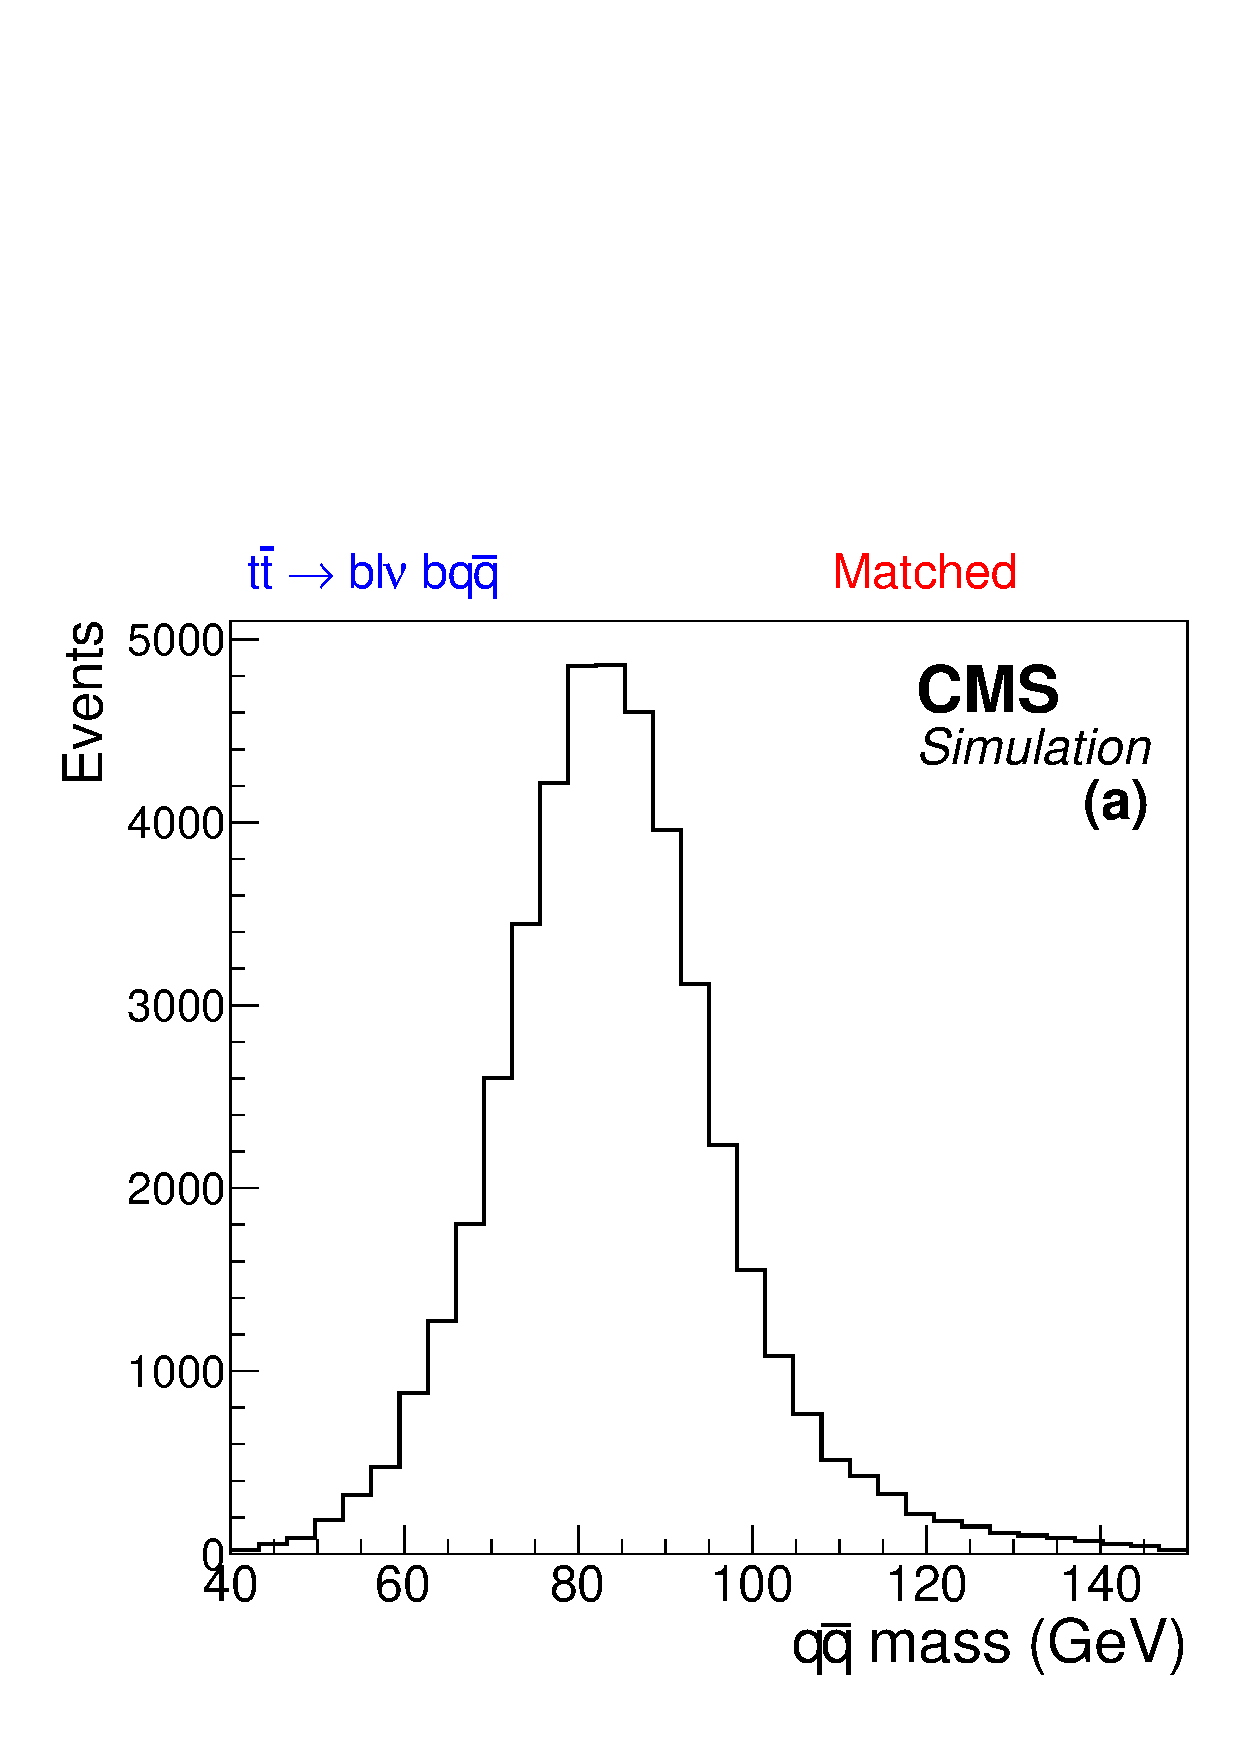
\includegraphics[width=\textwidth]{figures/dijet-matched}
    \caption{}
    \label{sfig:matched}
  \end{subfigure}%
  \begin{subfigure}{0.33\textwidth}
    \centering
    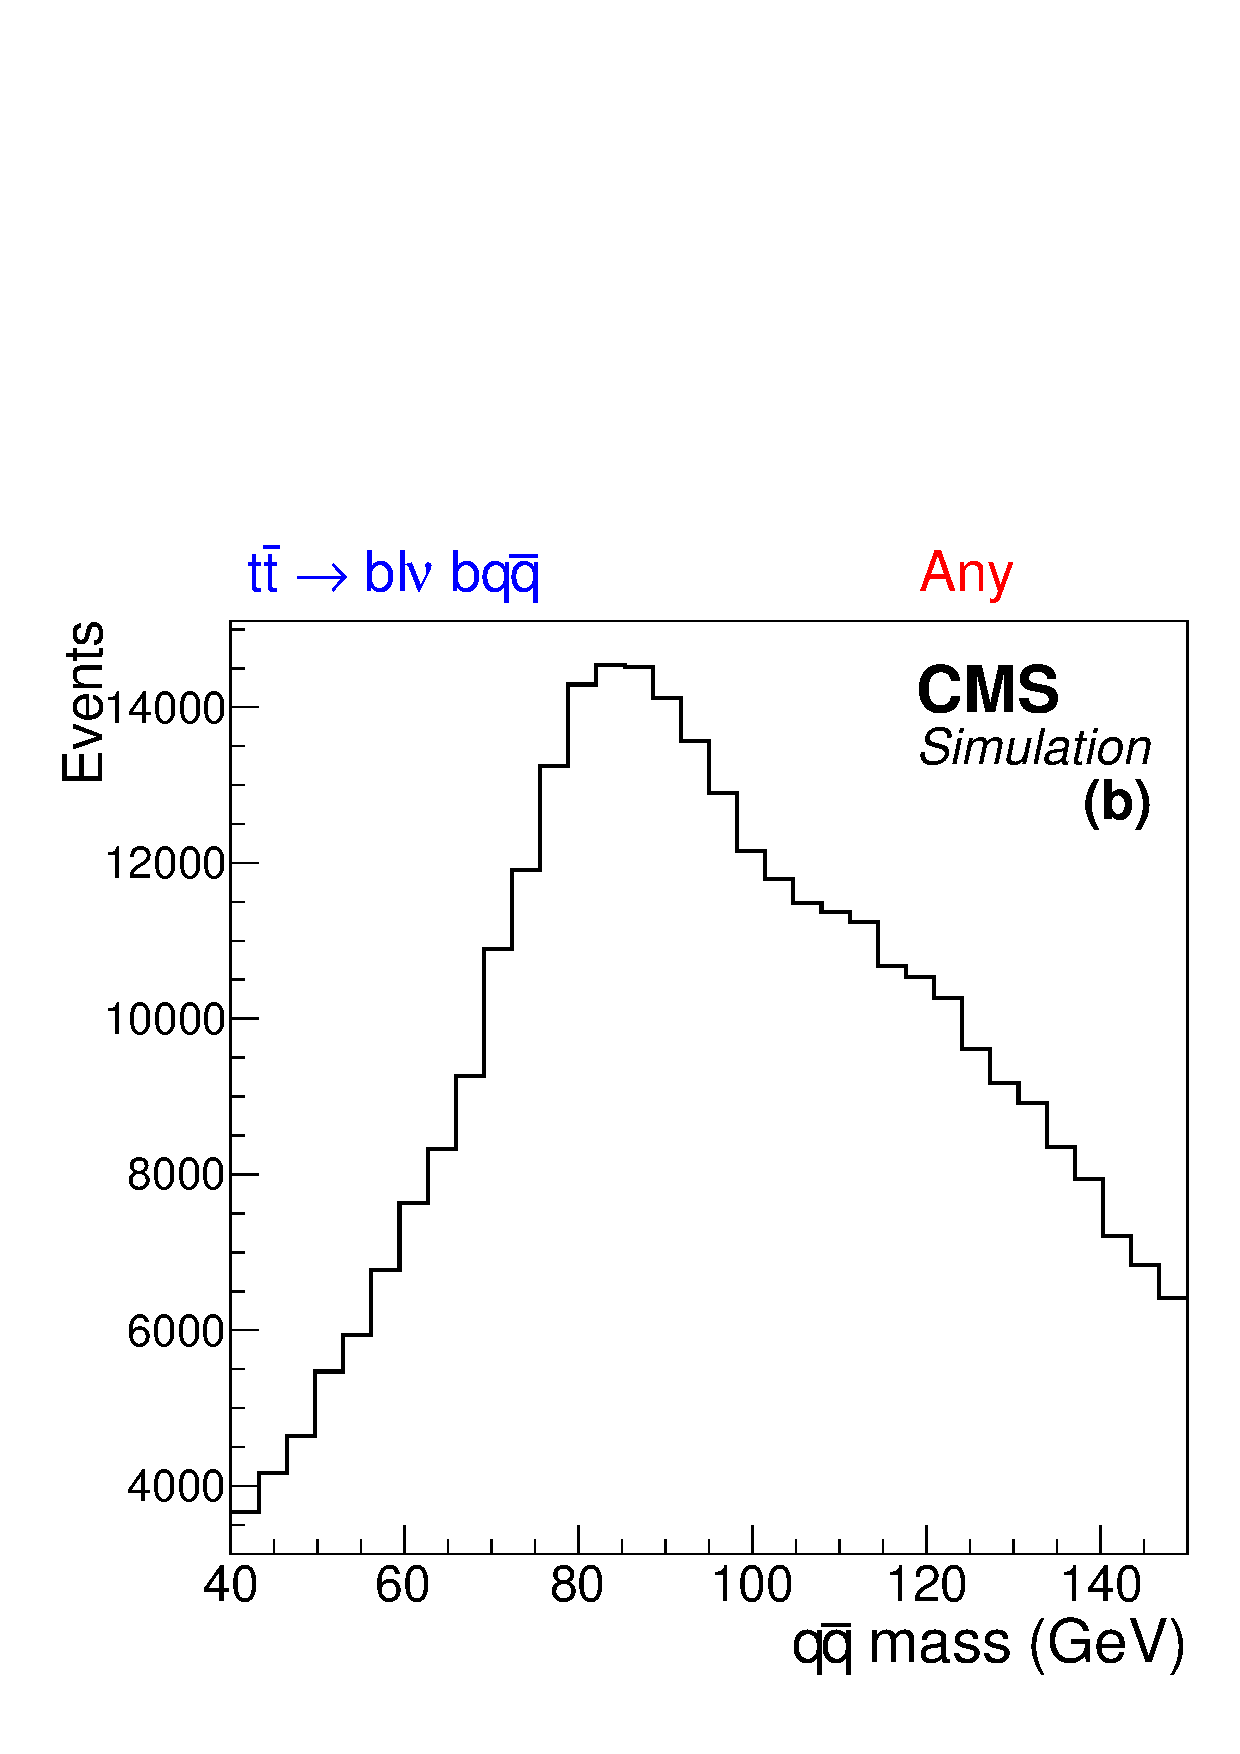
\includegraphics[width=\textwidth]{figures/dijet-any}
    \caption{}
    \label{sfig:any}
  \end{subfigure}%
  \begin{subfigure}{0.33\textwidth}
    \centering
    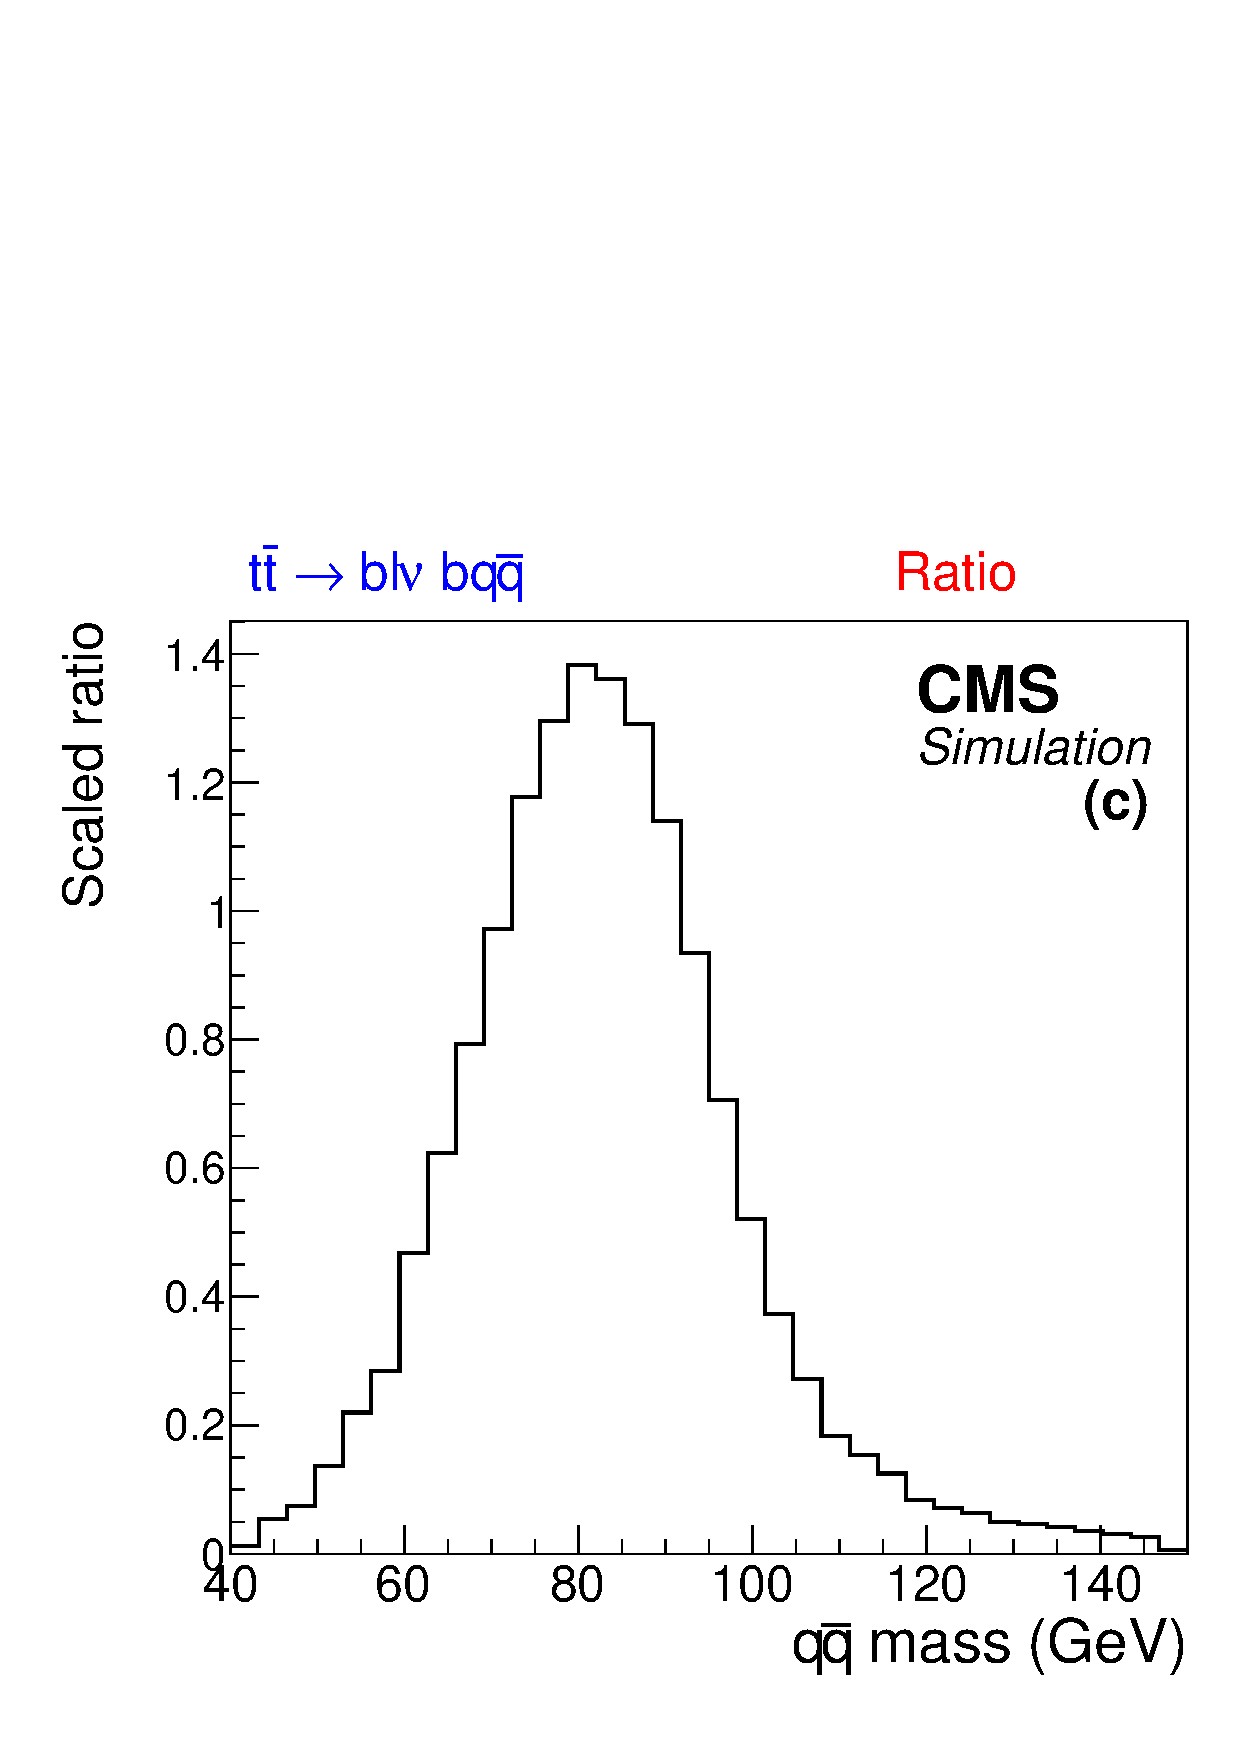
\includegraphics[width=\textwidth]{figures/dijet-ratio}
    \caption{}
    \label{sfig:ratio}
  \end{subfigure}%
  \caption[Dijet mass, for matched versus all possible dijet combinations]{
    The dijet mass in semileptonic \ttbar decays. In panel~\subref{sfig:matched},
    only pairs of jets arising from the decay of the same W are included. In
    panel~\subref{sfig:any}, no particular parentage is required; all dijet
    combinations are included. The ratio of the histograms in
    panels~\subref{sfig:matched} and~\subref{sfig:any} is presented
    in~\subref{sfig:ratio}.
  }
  \label{fig:match-ratio}
\end{figure}

\begin{table}
  \caption{Input variables to the full event reconstruction}
  \input{tables/eight-TeV/event_reco_match_score}
  \label{tab:event-reco-match-vars}
\end{table}

\section{Signal extraction}
\label{section:8_signal}
At this point, we had a set of events, each associated with a list of measured
input variables. We wished to assign each event to either signal or background
based on these measured parameters. To accomplish this end, we used a method called a
Boosted Decision Tree (BDT)~\cite{bdt_nim}.

A decision tree divides a set of events into two groups based on the cutoff values
for one or more parameters. The full sample, comprising equal parts signal and background
events, makes up the first \emph{node} of the tree. The sample is then divided using
the variable and cutoff value that provides the best discrimination between
signal and background events to create two \emph{branches}. These branches
become two new nodes, and the process is repeated until one of the stopping
criteria is satisfied; usually, a specified maximum number of final branches
(or \emph{leaves}) is obtained, a specified minimum number of events per branch
is reached, or a leaf is entirely signal or background. Finally, the tree
(\emph{trained} with simulated data, for which signal and background events are
labeled) can be used to assign a score to real (unlabeled) data events. Events
are fed through the tree, with each event following a path according to whether it passes or
fails each established cut. The event is then assigned a score based on the final leaf it
lands on, usually according to the purity (defined below) of the terminal leaf,
such that larger scores correspond to more signal-like events.

The quality of separation between signal and background events, designated
\emph{purity}, is defined as $P=\frac{\sum_sW_s}{\sum_sW_s+\sum_bW_b}$, where
each event has weight $W_i$ and $\sum_s$ refers to the sum over signal events
and $\sum_b$ refers to the sum over background events. Let the Gini index $G$ be
defined as $G=\sum_{i=1}^n W_i P(1-P)$. Note that $G=0$ if a sample is either
all signal or all background. To separate signal and background maximally, an
optimal cutoff value for a given input variable can be found by
minimizing $G_\text{pass} + G_\text{fail}$, where $G_\text{pass}$
($G_\text{fail}$) refers to the Gini index of the events that pass (fail) the
cut. The input variables can be ranked by finding the maximum value of
$G_\text{parent} - G_\text{pass} - G_\text{fail}$ for each one.

To improve performance, a \emph{boosting} procedure can be performed. After the
initial tree is built, the weight of misclassified events is increased and an
additional tree is constructed; this process is repeated many times to obtain a
\emph{forest} of trees. Events are fed through each tree, and the final
discriminant score is evaluated by summing the scores from all trees.

A total of 10 BDTs were generated, one for each jet category and channel, using
the ``gradient boosting" implementation in the Toolkit for Multivariate Analysis
package~\cite{Hocker:2007ht}. Simulated \ttW signal events were used with
simulated \ttbar background events for training of the SS \ttW and 3\lep \ttW
BDTs. Simulated \ttZ events were used with simulated \ttbar and WZ events for
the 3\lep \ttZ BDTs. For the OS \ttZ channel, we initially trained a BDT with \ttZ
events against a \ttbar background, then used that output as an input variable to
a final BDT, which was trained with \ttZ signal against \ttbar and Z boson
simulation. The 4\lep channel had too few events to train a BDT, so the number
of medium b-tagged jets was used as a discriminant instead. The match scores and
other input variables for all BDTs are listed
in~\crefrange{tab:BDT_inputs_SS_ttW}{tab:BDT_inputs_OS_ttZ}.

\input{tables/eight-TeV/bdt}
\section{Statistical procedure}
\label{sec:stats}
The procedure used to determine cross sections for \ttW and \ttZ is similar to
that used for the LHC Higgs boson analysis~\cite{Collaboration2012,
CMS-NOTE-2011-005}. The statistical analysis was based on previously described
methods~\cite{Beringer:1900zz, Cowan2011, BARLOW1990496}.

The quantum mechanical nature of events produced at the LHC is such that the
outcome is characterized by \textit{random variables}; that is, the result of a
single event cannot be predicted deterministically even if the parameters, $H$,
of the Lagrangian describing the system are completely known. With
complete knowledge of $H$, however, accurate predictions can be made about
the statistical distribution of the outcomes of a large number of such
experiments. The description of the statistical distribution of a random
variable is called a probability density function; an integral of a probability
density function for some variable over some interval results in the probability
of the variable having a value that falls within that interval.

In experimental studies, however, we are often faced with the opposite
situation. We can conduct an experiment hundreds or thousands of times and
observe the statistical distribution of the outcome. However we do not,
\textit{a priori}, know the parameters $H$ of the hypothesized mechanism. How
can we decide what value for $H$ represents the best possible description of the
physical system?

To answer this question, we can utilize two similar but distinct functions.
Consider a hypothesis characterized by one or more parameters $H$. Given $H$,
the probability of obtaining an outcome $x$ is known as the probability density
function $p(x|H)$. Often, however, $H$ is unknown; we instead observe $x$ and
try to determine the most plausible $H$ (note that we are now viewing $x$ as a
function of $H$). A natural choice is to choose $H$ such that the probability of
observing $x$ is maximized; that is, we maximize the likelihood function $L(H)$,
defined as $L(H) = p(x|H)$.

A likelihood function is constructed as follows. Denote the expected number of
signal events predicted by the SM as $s$, and the expected number of background
events as $b$. We introduce the signal strength modifier
$\mu=\frac{\sigma}{\sigma_\text{SM}}$, such that $\mu=0$ corresponds to the
background-only hypothesis, and $\mu=1$ corresponds to the SM hypothesis. The
total number of expected events is $\mu s + b$. The likelihood function is the
conditional probability of obtaining the observed number of data events
$n_{obs}$ given that we expect $\mu s + b$ events.

\clearpage
The number of observed events $n_i$ for each bin $i$ of the final discriminant
in each channel follows a Poisson distribution with mean $\mu s_i + b_i$. The
$n_i$ are statistically independent, so the likelihood
function\footnote{Technically, this is the extended likelihood
function~\cite{BARLOW1990496}. The standard maximum likelihood method maximizes
$L = \prod_{i=1}^M p(x_i; a_1..a_n)$ where $p$ is the probability density
(normalized to 1), M is the number of events, $x$ is the measured quantity, and
$a_i$ are the parameters to be determined. The fit only determines the shape and
indicates nothing about the number of events. In the extended maximum likelihood, the
predicted $N$ is a function of the parameters, and the fit determines shape and
size: $p$ is replaced by $P$ with $\int P(x_i| a_1..a_n)dx_i = N(a_1..a_n)$. For
example, say the lifetime of a light bulb is modeled by an exponential
distribution with lifetime $\lambda$. The lifetime $x$ of M light
bulbs can be tested and the result used to calculate the maximum likelihood estimate of $\lambda$. In
this case, M is not dependent on $\lambda$, and the probability
$p(x|\lambda)=\lambda e^{-\lambda x}$ must be normalized to 1 (if a
measurement is made, \emph{some} lifetime will be observed). For our cross section
measurements, on the other hand, the number of observed events itself is
relevant to the cross section being measured, so it should appear in the
likelihood function.} is the product of Poisson probabilities over $M$ bins:
\begin{equation}
  L(\mu) = \prod_{i=1}^{M} \frac{(\mu s_i + b_i)^{n_i}}{n_i!} e^{-(\mu s_i + b_i)}.
\end{equation}
Various uncertainties are associated with our model. We introduce a
\emph{nuisance parameter} to parameterize each uncertainty and denote the set
as $\theta$; the expected signal and background yields become $s(\theta)$ and
$b(\theta)$. When channels have the same uncertainty, it is represented with the
same nuisance parameter. This correlation allows for bins in \emph{control
regions} with many data events but few expected signal events to constrain large
uncertainties. The conditional probability to measure a nuisance parameter to be
$\widetilde{\theta_i}$, given that the true value is $\theta_i$, is encoded in
the probability density function $\rho(\widetilde{\theta_i}|\theta_i)$. For
uncertainties that must be positive (like cross sections and luminosities),
a log-normal distribution for $\rho$ is typically used. For statistical uncertainties
on the number of events in a control region, we usually use the gamma
distribution. Denoting the probability density function for the full set of
nuisance parameters as $\rho(\widetilde{\theta}|\theta)$, we have the following:
\begin{equation}
  \label{eq:likelihood}
  L(\mu, \theta) = \mathcal{P}(\text{data}|\mu, \theta)\rho(\widetilde{\theta}|\theta) = \prod_{i=1}^{M} \frac{(\mu s_i + b_i)^{n_i}}{n_i!} e^{-(\mu s_i + b_i)} \rho(\widetilde{\theta}|\theta).
\end{equation}

We denote $\hat{\theta}$ and $\hat{\mu}$ to be the values of $\theta$ and $\mu$
that globally maximize $L$, referred to also as the best fit (or post-fit)
values. But $\hat{\mu}$ by itself cannot reveal the whole story. We have found the
best $\mu$ \emph{relative} to the other possible ones our model permits, but
it may just be the best choice from among very bad choices. We
wish to define some scalar function of the data whose value encodes the level of
compatibility between the data and a hypothesized value of $\mu$. Furthermore,
we wish to remove the dependence on the nuisance parameters. We can accomplish
this approximately by making use of the \emph{profile likelihood ratio}, which
is only a function of $\mu$:
\begin{equation}
\label{eq:likelihoodratio}
\lambda(\mu) = \frac{L(\mu, \doublehat{\theta}(\mu))}{L(\hat{\mu}, \hat{\theta})}
\end{equation}
where $\doublehat{\theta}(\mu)$ is the value of $\theta$ that maximizes $L$ for
a given $\mu$ (and thus a function of $\mu$ itself). The profile likelihood can
take on values $0 \leq \lambda \leq 1$, with higher $\lambda$ implying better
agreement with the data. Noting that the log of a function will be maximized at
the same point as the function itself, we can equivalently define the test
statistic\footnote{Sometimes the quantity $\ln\lambda=\ln L(\mu,\doublehat{\theta}(\mu)|\text{data})-\ln L(\hat{\mu}, \hat{\theta}|\text{data})$
is referred to as $\Delta \ln L$.} $t_\mu=-2\ln \lambda(\mu)$, which,
according to Wilks' theorem, has the advantage of approaching a $\chi^2$ distribution
for large data samples independently of $\theta$~\cite{Cowan2011}. As $t_\mu$
gets larger, the incompatibility between the data and $\mu$ increases. In this
analysis, we wish to determine if we have discovered a signal. We consider $\mu$
to be physically bounded by $\mu \geq 0$, and we want to reject the
background-only hypothesis that $\mu=0$, so we define
\begin{equation}
  \label{eq:q0}
  q_{0} =
  \left\{ \! \! \begin{array}{ll}
      - 2 \ln \lambda(0) = -2 \ln \frac{L(\doublehat{\theta}(0))}{L(\hat{\mu}, \hat{\theta})}
      & \quad \hat{\mu} \ge 0 \;, \\
      0 & \quad \hat{\mu} < 0  \;,
    \end{array}
  \right.
\end{equation}
where $\doublehat{\theta}(0)$ correspond to the nuisance parameter values that
maximize $L$ under the background-only hypothesis. As the yield gets larger than
the background, the incompatibility between the data and the
background-only hypothesis increases. We now calculate the p-value
\begin{equation}
  \label{equation:p0}
  p_0 = P(q_0 \geq q_0^\text{obs}) = \int_{q_0^\text{obs}}^\infty f(q_0|0) dq_0,
\end{equation}
which reveals what the probability that $q_0$ would be at least as large as
the one we observe, $q_0^\text{obs}$, under the background-only hypothesis; in
other words, it is the probability that the background events look as
signal-like as those in the data. We define the significance $Z$ such that
the probability is $p_0$ to find a Gaussian distributed variable $Z$ standard
deviations $\sigma$ above the mean:
\begin{equation}
  \label{equation:Z}
  p_0 = \int_Z^\infty \frac{1}{\sqrt{2\pi}}e^{-x^2/2}dx.
\end{equation}
\todo[inline]{for explanation of significance Z see figure 1 https://arxiv.org/pdf/1007.1727.pdf}

In high energy physics, the convention is to consider $Z=5$, corresponding to $p =
\num{2.87e-7}$, as the threshold for discovery. In other words, a discovery
corresponds to an observation that, to be consistent with the
background-only hypothesis, would require a statistical fluctuation that is
expected to occur fewer than three times out of every 10 million otherwise
identical experiments.

To evaluate~\cref{equation:p0}, we need to know $f(q_0|0)$. We could generate MC
pseudo-data by sampling from $\mathcal{P}(\text{data}|\mu, \theta)$ and
$\rho(\widetilde{\theta}|\theta)$ around $\mu=0$; however, we instead use the
approximation from~\cite{Cowan2011}, which draws on the fact that $f(q_0|0)$
approximates a $\chi^2$ distribution for large datasets.

We would also like to determine confidence intervals; in other words, ranges of
possible values of $\mu$ that have a given probability of containing the true
value of $\mu$. Quantifying the absence of a signal will be required, so we
consider a closely related test statistic:
\begin{equation}
  \label{eq:qmu}
  q_{\mu} =
  \left\{ \! \! \begin{array}{ll}
    - 2 \ln \lambda(\mu) & \quad \hat{\mu} \leq \mu \;, \\
               0 & \quad \hat{\mu} > \mu  \;.
  \end{array}
       \right.
\end{equation}

We require that $q_\mu=0$ when $\hat{\mu} > \mu$ so that upward fluctuations of
the data such that $\hat{\mu} > \mu$ are not considered evidence against the
signal hypothesis. Denoting the cumulative distribution function of $q_\mu$ as
$F(q_\mu|\mu)$, the p-value is
\begin{equation}
  p_\mu = P(q_\mu \geq q_\mu^\text{obs}) = 1 - F(q_\mu|\mu) =
  \int_{q_\mu^\text{obs}}^\infty f(q_\mu|\mu) dq_\mu.
  \label{equation:pmu}
\end{equation}
If $p_\mu \leq \alpha$ for a specified probability $1 - \alpha$, then the
corresponding $\mu$ is said to be excluded with a confidence level (CL) of
$1-\alpha$, and the set of points that is not excluded create the $1 - \alpha$ CL
interval. We can find the endpoints of the interval by setting $p_\mu=\alpha$
and solving for $\mu$. Recall that $2 \ln \lambda = 2 \Delta \ln L$ approaches
the $\chi^2$ distribution with $n$ degrees of freedom for large samples, where
$n$ is the number of parameters being estimated:
\begin{equation}
  1 - \alpha = 1 - p_\mu = F(q_\mu|\mu) \approx (\chi^2;n).
  \label{eq:cl}
\end{equation}
We can then find the interval endpoints by evaluating the quantile function
(the inverse of the cumulative distribution function) $F^{-1}(1 - \alpha)$. For
estimations with one degree of freedom, a \SI{68.27}{\percent} CL corresponds to
$-2\Delta \ln L = 1.00$ and a \SI{95}{\percent} CL corresponds to $-2\Delta \ln
L = 3.84$.
% https://arxiv.org/pdf/1007.1727.pdf
%
\section{Systematic uncertainties}
\label{sec:8-systematics}
The use of nuisance parameters for encoding uncertainties was introduced in
~\cref{sec:stats}. In the current section, the various sources of systematic
uncertainties are discussed in more detail. Unlike statistical
uncertainties, systematic uncertainties do not get smaller as more data are
accrued. Systematic uncertainties arise from uncertainties in the measurement
process and theoretical models, for example, because of imperfectly known detector
performance, discriminant efficiencies, and SM parameters. We must examine the
associated uncertainties and how they affect the final determination of cross
sections of the various channels. For \ttW, the largest uncertainties come from
the CSV shape, theoretical uncertainties in the signal modeling, and the rate of
nonprompt backgrounds. For \ttZ, the largest uncertainties are associated with
the CSV shape, signal modeling, and the rates of nonprompt backgrounds and
prompt Z, WZ, and ZZ with extra jets. \emph{Rate uncertainties} affect the rate
of a process, which alters each bin of the final discriminant by the same value.
\emph{Shape uncertainties} affect the shape of variables and can alter bins
separately, changing the shape of the discriminant.

\begin{description}
  \item[Integrated luminosity and pileup] There was a \SI{2.6}{\percent}
    uncertainty on the integrated luminosity~\cite{CMS-PAS-LUM-13-001}, which
    was
    correlated across the entire analysis. The total inelastic proton--proton
    cross section was varied up and down by \SI{5}{\percent}, which affected the
    number of pileup vertices, and was propagated to the output
    distributions~\cite{tagkey20135}.
  \item[Jet energy scale] To account for uncertainty on the energy assigned to
    jets (the jet energy scale, or JES~\cite{cmsJEC}), we computed the MC with
    the JES shifted up and down by one standard deviation and used the resulting
    rates and distributions to define the uncertainty.
  \item[b tagging efficiency] We estimated the number of non-b jets in the data
    region used to derive the b jet CSV shape. We also estimated the number of bottom and
    charm jets in the data region used to derive the event weights for
    light-flavor jets. The uncertainties associated with those estimates were
    assessed by shifting the expected yields of contaminated jets up and down by
    one standard deviation. An additional source of uncertainty was associated
    with the finite number of data events used to calculate the individual
    weights in each bin of \pT, $\eta$, CSV, and flavor. We approximated these
    by
    using an \emph{envelope} of maximum linear and quadratic shifts. The linear
    shift for a given bin was given by $f_l = \sigma (1 - 2x)$, where $x$ was the
    central CSV value of the bin and $\sigma$ represents the statistical
    uncertainty on that bin. The quadratic shift corresponded to $f_q = \sigma (1
    - 6x + 6x^2)$. The SFs for each bin were then shifted within the envelope
    defined by $\pm f_l$ and $\pm f_q$. Uncertainties were not separately derived
    for c jets, rather they were assigned an uncertainty twice that of the b
    jets.
  \item[Selection efficiency for prompt leptons] There was uncertainty associated
    with the SFs used to correct for differences in reconstruction and selection
    efficiency for prompt leptons between the data and MC. Because the calibration
    region had so many events, these uncertainties were small. There was
    uncertainty associated with the efficiency to reconstruct and select prompt
    leptons of \SI{1.5}{\percent} per lepton. The dilepton trigger efficiencies
    had an associated \SI{3}{\percent} uncertainty in the rate, while
    three-lepton events had an associated \SI{1}{\percent} rate uncertainty.
    Four-lepton events had no trigger efficiency uncertainty.
  \item[Selection efficiency for nonprompt leptons] A \SI{40}{\percent}
    uncertainty was assigned to the rate of nonprompt electrons and a
    \SI{60}{\percent} uncertainty to the rate of nonprompt muons passing the
    tight selection, based on the agreement between expected and observed yields
    in control regions. Most nonprompt leptons have low \pT, so uncertainties of
    \SI{50}{\percent} were applied to the rates of \SIrange{20}{30}{\GeV} muons
    and \SIrange{20}{40}{\GeV} electrons, and an additional \SI{100}{\percent}
    to muons with $\pT > \SI{30}{\GeV}$ and electrons with $\pT >
    \SI{40}{\GeV}$. Because the SS and 3\lep channels may have different sources
    of nonprompt leptons, the uncertainties were applied separately for
    electrons and muons, and were uncorrelated between the SS and 3\lep channels. The
    final discriminant contained bins with mostly nonprompt backgrounds; such
    bins were useful in order to constrain these uncertainties. The final fit
    constrained them to \SIrange{10}{15}{\percent}.
  \item[Rate of charge misidentified electrons] In the SS channel, a
    \SI{30}{\percent} rate uncertainty was assessed on the rate of charge
    misidentified electrons based on the level of agreement in the control
    region of SS ee events consistent with a Z boson decay.
  \item[Top quark \pT reweighting] To assess the uncertainty due to the top
    quark \pT reweighting of \ttbar MC, we obtained a lower bound by removing the \pT
    weighting, and an upper bound by assessing twice the weight.
  \item[Prompt backgrounds with extra HF jets] Rate uncertainties were applied to
    account for the SFs applied to correct the yields in Z events with five or
    more jets and in WZ and ZZ events with three or more jets; these uncertainties
    were relatively large because of the relatively small number of events in the
    light-flavor control region. Events with a Z boson plus five jets or six or
    more jets received uncorrelated \SI{30}{\percent} rate uncertainties. WZ and
    ZZ events received a \SI{40}{\percent} uncertainty if they had three jets,
    and a \SI{60}{\percent} uncertainty if they had four or more jets. The
    Z+\ccbar, Z+b, and Z+\bbbar uncertainties were constrained to
    \SI{30}{\percent} each, owing to good agreement in dileptonic Z boson events
    with four jets. To account for the deviations between data and MC seen in Z
    boson events with four or more jets (excluding the \ttZ signal region) in
    the distribution of \HTmiss, an additional shape uncertainty was added by
    weighting events by $w = 1 \pm 0.005(\HTmiss - 30)$. Mismodeling was also
    observed in the ratio between the \MT and the invariant mass of the
    reconstructed jets and leptons in an event. This variable measured the
    centrality of the Z boson decay products. To account for this deviation, an
    additional shape uncertainty was added by weighting events by $w = 1.0 \pm
    0.7(\frac{\MT}{\text{mass}} - 0.65)$. A control region of OS $e\mu$ events
    with five or more jets showed similar mismodeling in the \MT-to-mass ratio,
    so the same shape uncertainty was applied to \ttbar events.
  \item[PDF uncertainties] A rate uncertainty associated with the choice of PDF
    of \SI{7.2}{\percent} for \ttW and \SI{8.2}{\percent} for \ttZ was
    assessed~\cite{Alekhin:2011sk, Botje:2011sn}. In addition, shape
    uncertainties derived by using different PDF sets and \pythia tunes were
    applied to \ttW, \ttZ, and \ttH using envelope shape uncertainties of
    \SIrange{10}{11}{\percent}.
  \item[Renormalization and factorization scales] There was a rate uncertainty of
    \SI{10}{\percent} for \ttW and \SI{11}{\percent} for \ttZ, associated with
    the choice of renormalization and factorization
    scales~\cite{Garzelli:2012bn}.
  \item[Rare processes] Expected yields are small for rare processes, including
    WWW, WWZ, tbZ, $\ttbar\gamma$/$\ttbar\gamma^{*}$, and $\ttbar\PW\PW$. These
    have not yet been measured, and some have not been calculated at NLO.
    Consequently,
    they received conservative \SI{50}{\percent} rate uncertainties.
\end{description}

\section{Results}
The expected signal and background yields, obtained by performing the fit
described in~\cref{sec:stats}, are presented
in~\cref{tab:yields_OS,tab:yields_SS,tab:yields_3l_4l}.

We performed a one-dimensional fit for the \ttW cross sections, with the \ttZ
cross section set to the SM prediction with an uncertainty equal to the
uncertainty in the theory prediction, and vice versa. The $\ttZ$ cross section
was measured to be $242^{+65}_{-55}\text{fb}$ with a significance of 6.4 standard
deviations from the background-only hypothesis, which agrees well with the SM
prediction. The $\ttW$ cross section was higher than expected, measured to be
$382^{+117}_{-102}\text{fb}$ with a significance of 4.8 standard deviations from
the background-only hypothesis. The discrepancy was driven by an excess of SS
dimuon data events. A similar excess was seen in the CMS \ttH
search~\cite{Khachatryan2014ttH}, also mostly due to the same dimuon events. No
evidence of mismodeling was found. The best fit values were compatible with the
SM expectation at the \SI{13}{\percent} CL for \ttW and at the \SI{60}{\percent}
level for \ttZ. These results are summarized
in~\cref{tab:8-results-ttZ,tab:8-results-ttW}. The post-fit plots, which have
the nuisances and signal strengths set to their best fit values, are presented
in~\cref{fig:8-postfit-bdt-ttW,fig:8-postfit-bdt-ttZ}.

We also used all channels to perform a fit to both of the \ttW and \ttZ cross
sections simultaneously. The two-dimensional likelihood scan in $(\sigma_{\ttZ},
\sigma_{\ttW})$ plane is presented in~\cref{fig:8-2d-ttZ-ttW}. The best fit
values from the simultaneous fit are close to those for the one-dimensional fits
and compatible with the SM at the \SI{15}{\percent} CL.

\begin{table}
  \input{tables/eight-TeV/yields_OS}
\end{table}
\begin{landscape}
  \begin{table}
  \vspace{-2cm}
    \input{tables/eight-TeV/yields_SS}
  \end{table}
\end{landscape}
\begin{landscape}
  \begin{table}
  \vspace{-2cm}
    \input{tables/eight-TeV/yields_3l_4l}
  \end{table}
\end{landscape}

\begin{table}
  \input{tables/eight-TeV/results_ttW}
  \label{tab:8-results-ttW}
\end{table}
\begin{table}
  \input{tables/eight-TeV/results_ttZ}
  \label{tab:8-results-ttZ}
\end{table}
\begin{figure}[tb]
  \begin{subfigure}{0.33\textwidth}
    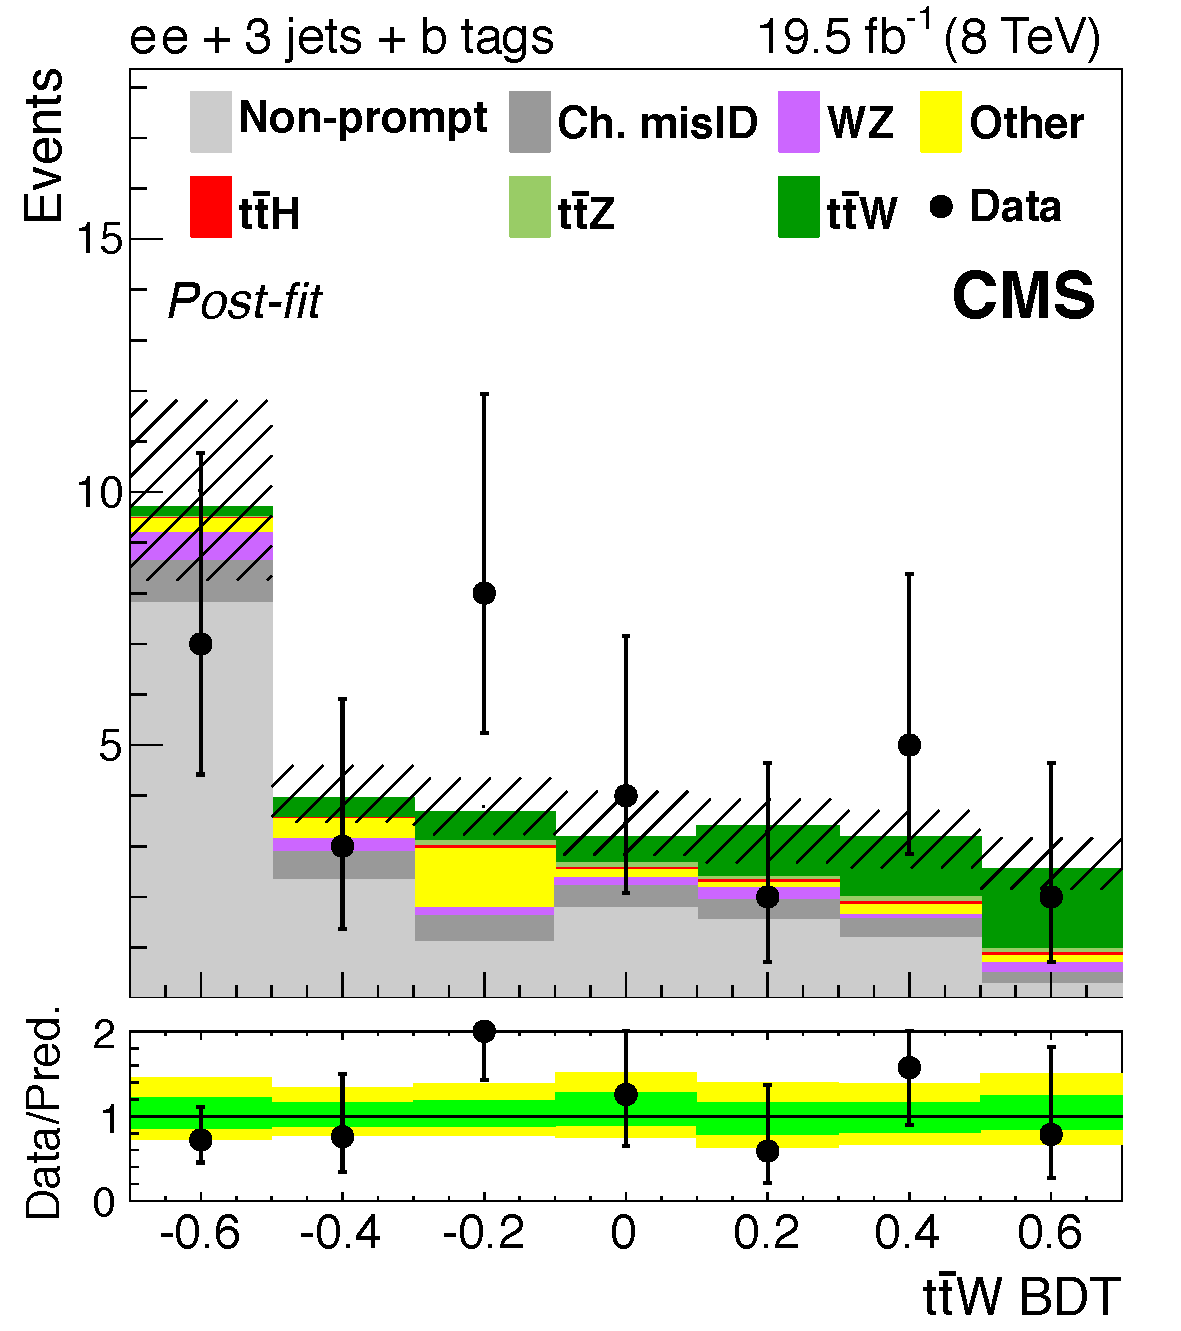
\includegraphics[width=\textwidth]{figures/eight-TeV/mva/ele_ele_eq3j_bloose_FinalBDT}
    \caption{}
    \label{sfig:8-ttW-tl}
  \end{subfigure}%
  \begin{subfigure}{0.33\textwidth}
    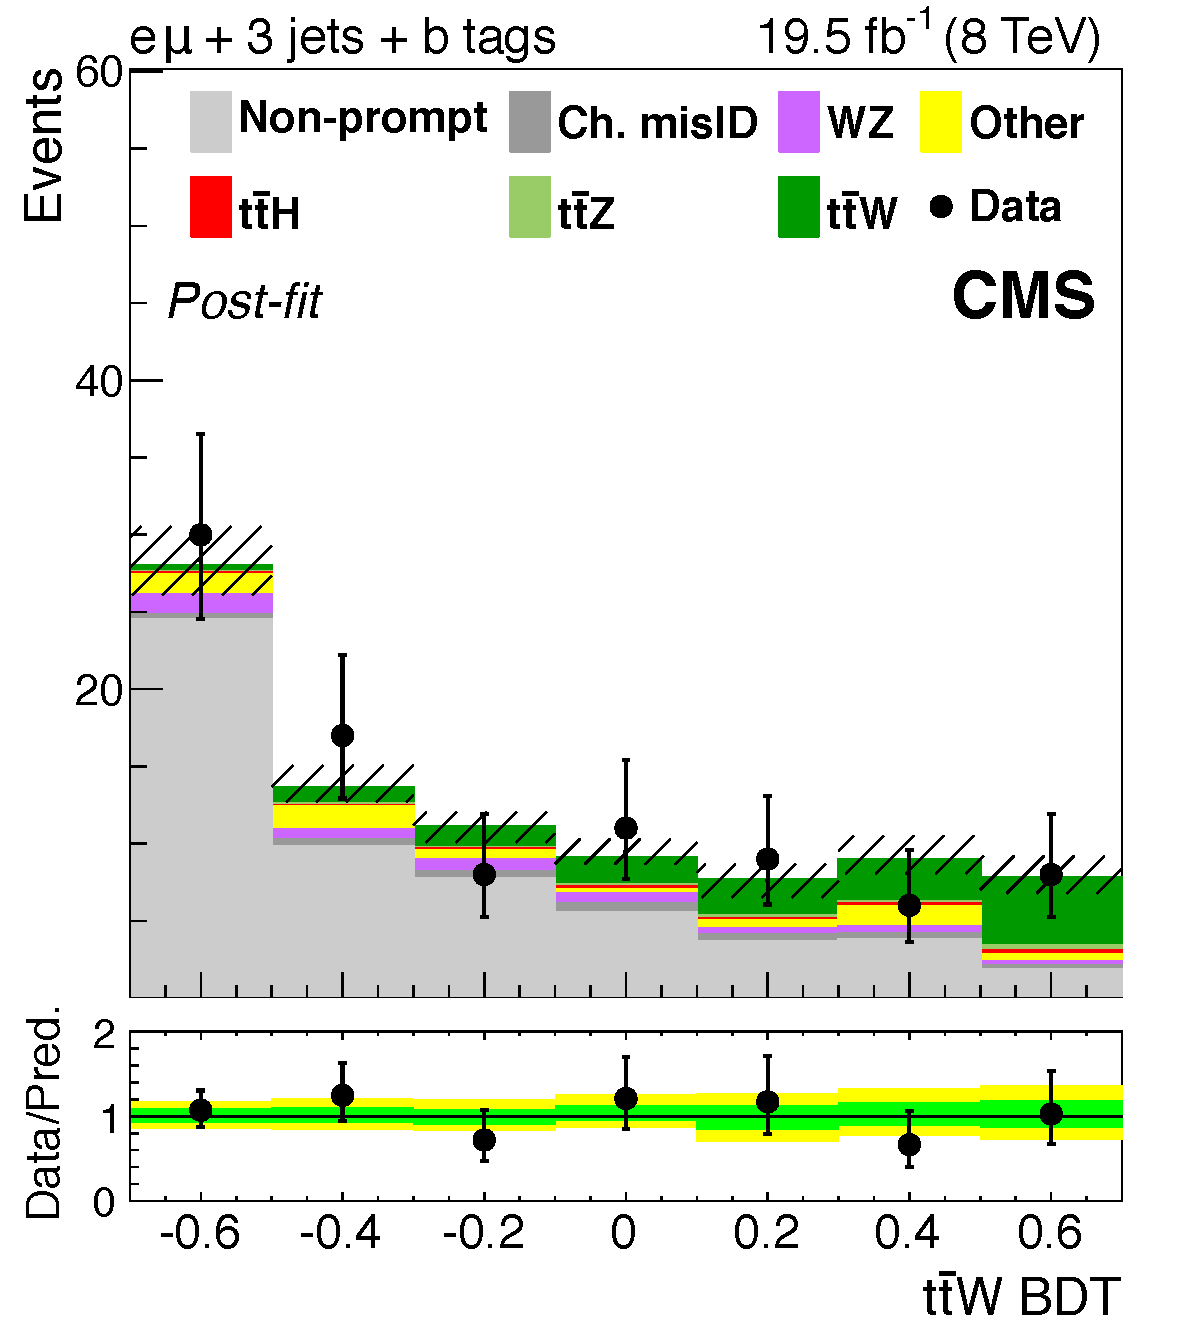
\includegraphics[width=\textwidth]{figures/eight-TeV/mva/mu_ele_eq3j_bloose_FinalBDT}
    \caption{}
    \label{sfig:8-ttW-tc}
  \end{subfigure}%
  \begin{subfigure}{0.33\textwidth}
    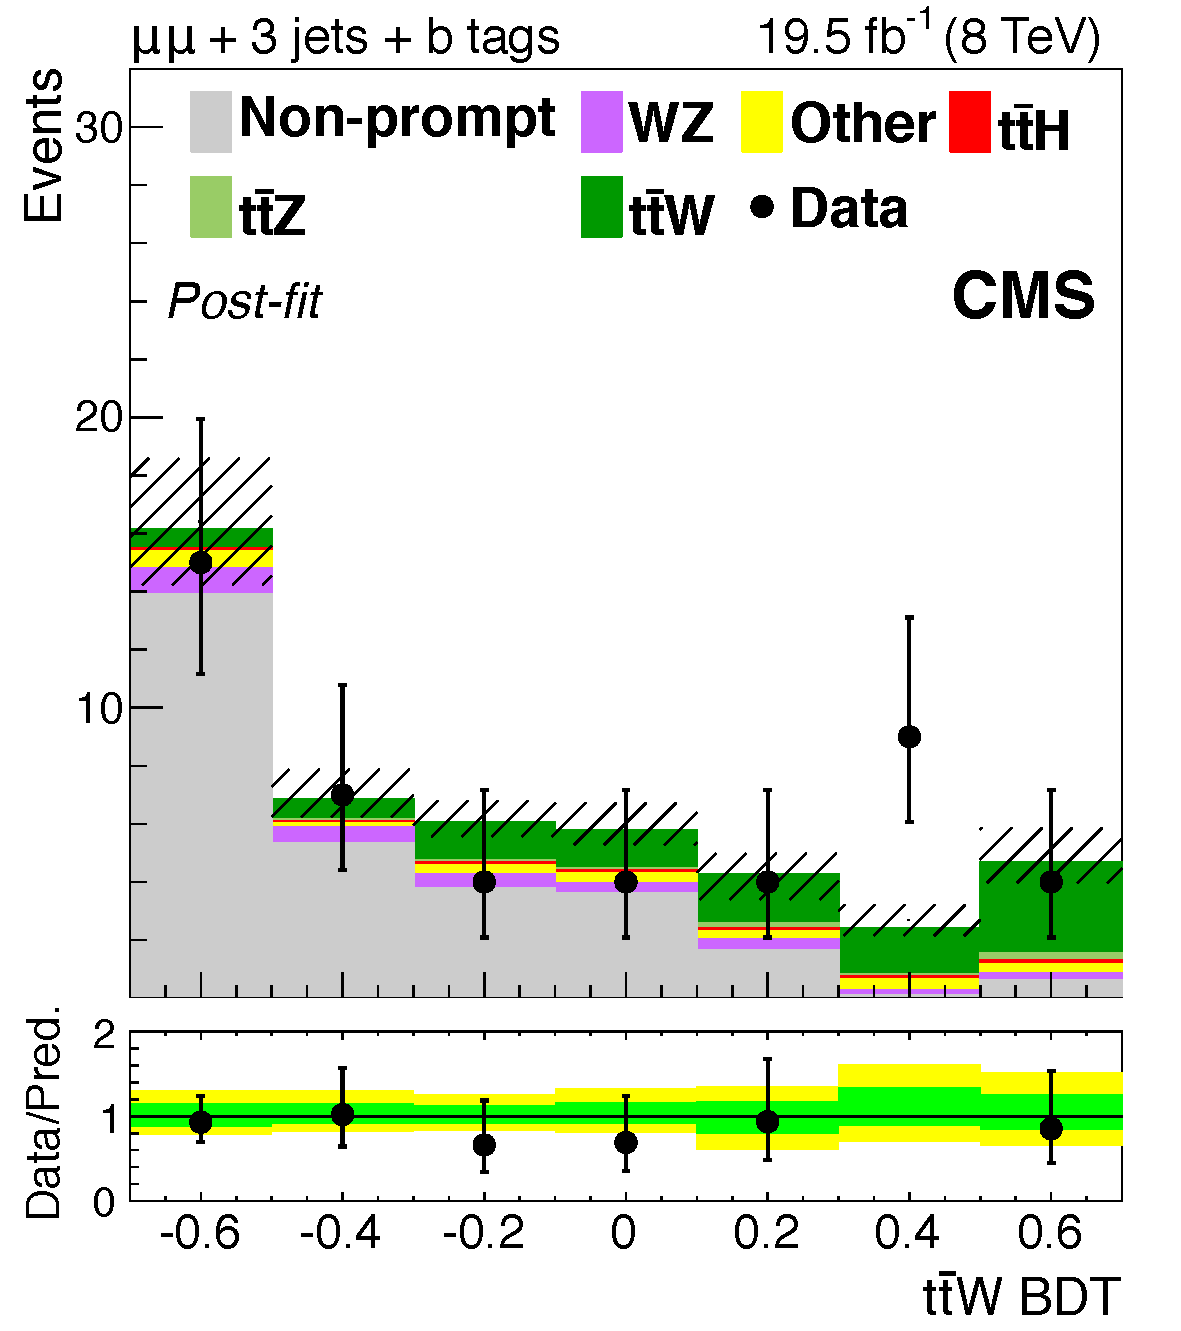
\includegraphics[width=\textwidth]{figures/eight-TeV/mva/mu_mu_eq3j_bloose_FinalBDT}
    \caption{}
    \label{sfig:8-ttW-tr}
  \end{subfigure}
  \begin{subfigure}{0.33\textwidth}
    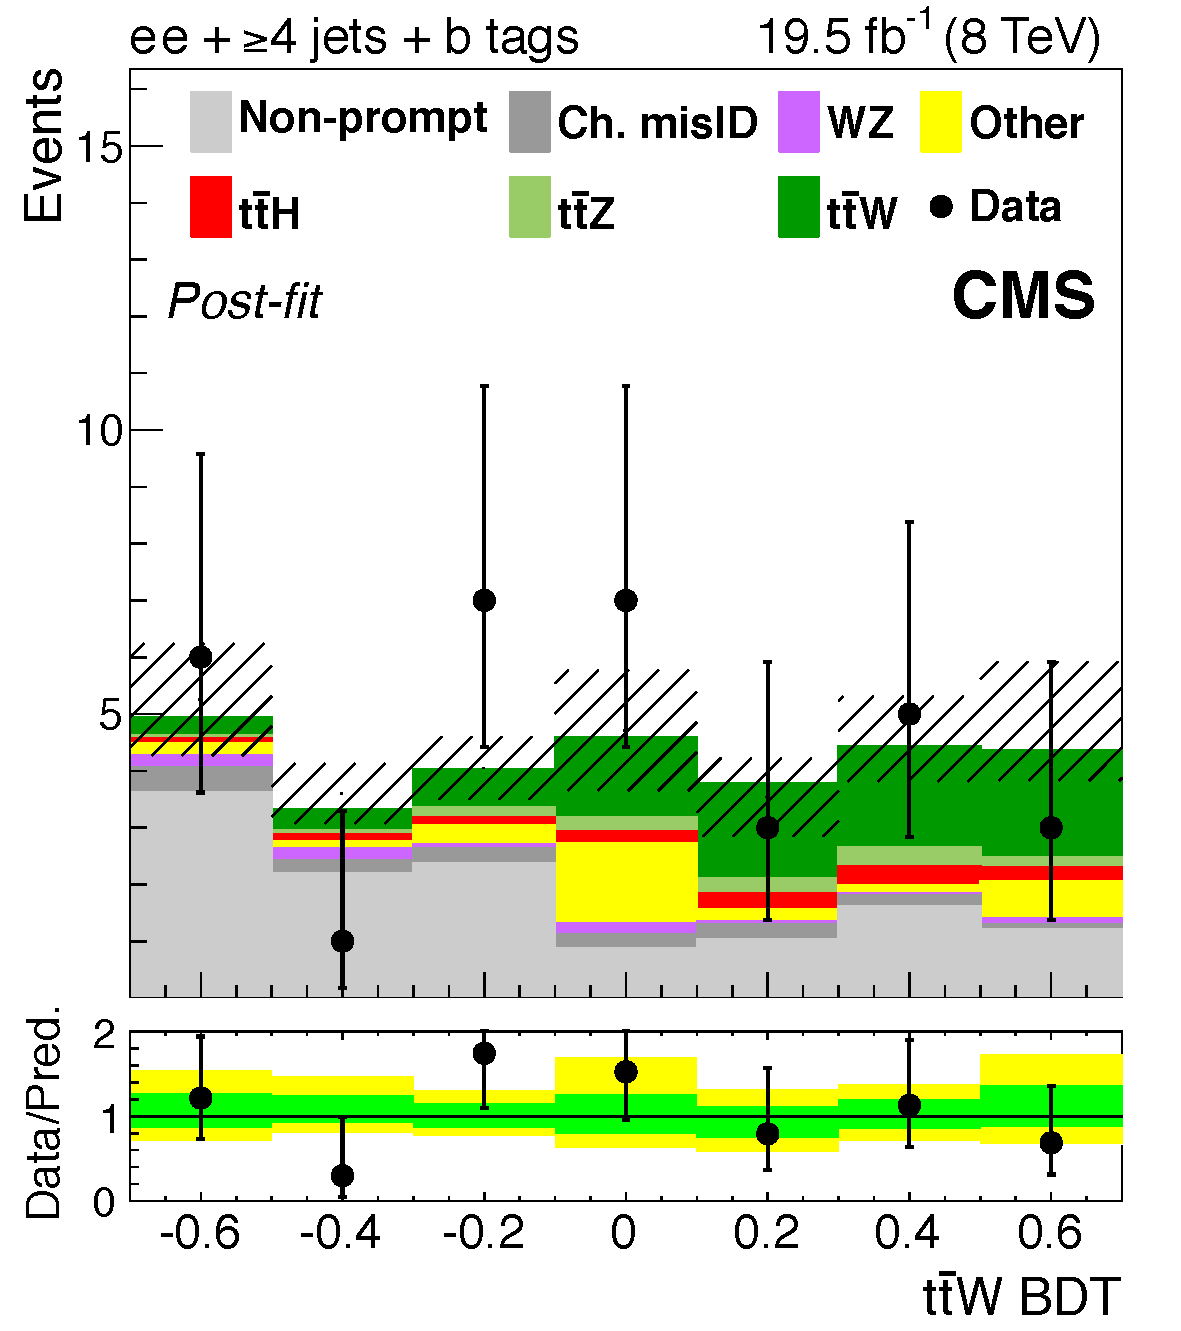
\includegraphics[width=\textwidth]{figures/eight-TeV/mva/ele_ele_ge4j_bloose_FinalBDT}
    \caption{}
    \label{sfig:8-ttW-cr}
  \end{subfigure}%
  \begin{subfigure}{0.33\textwidth}
    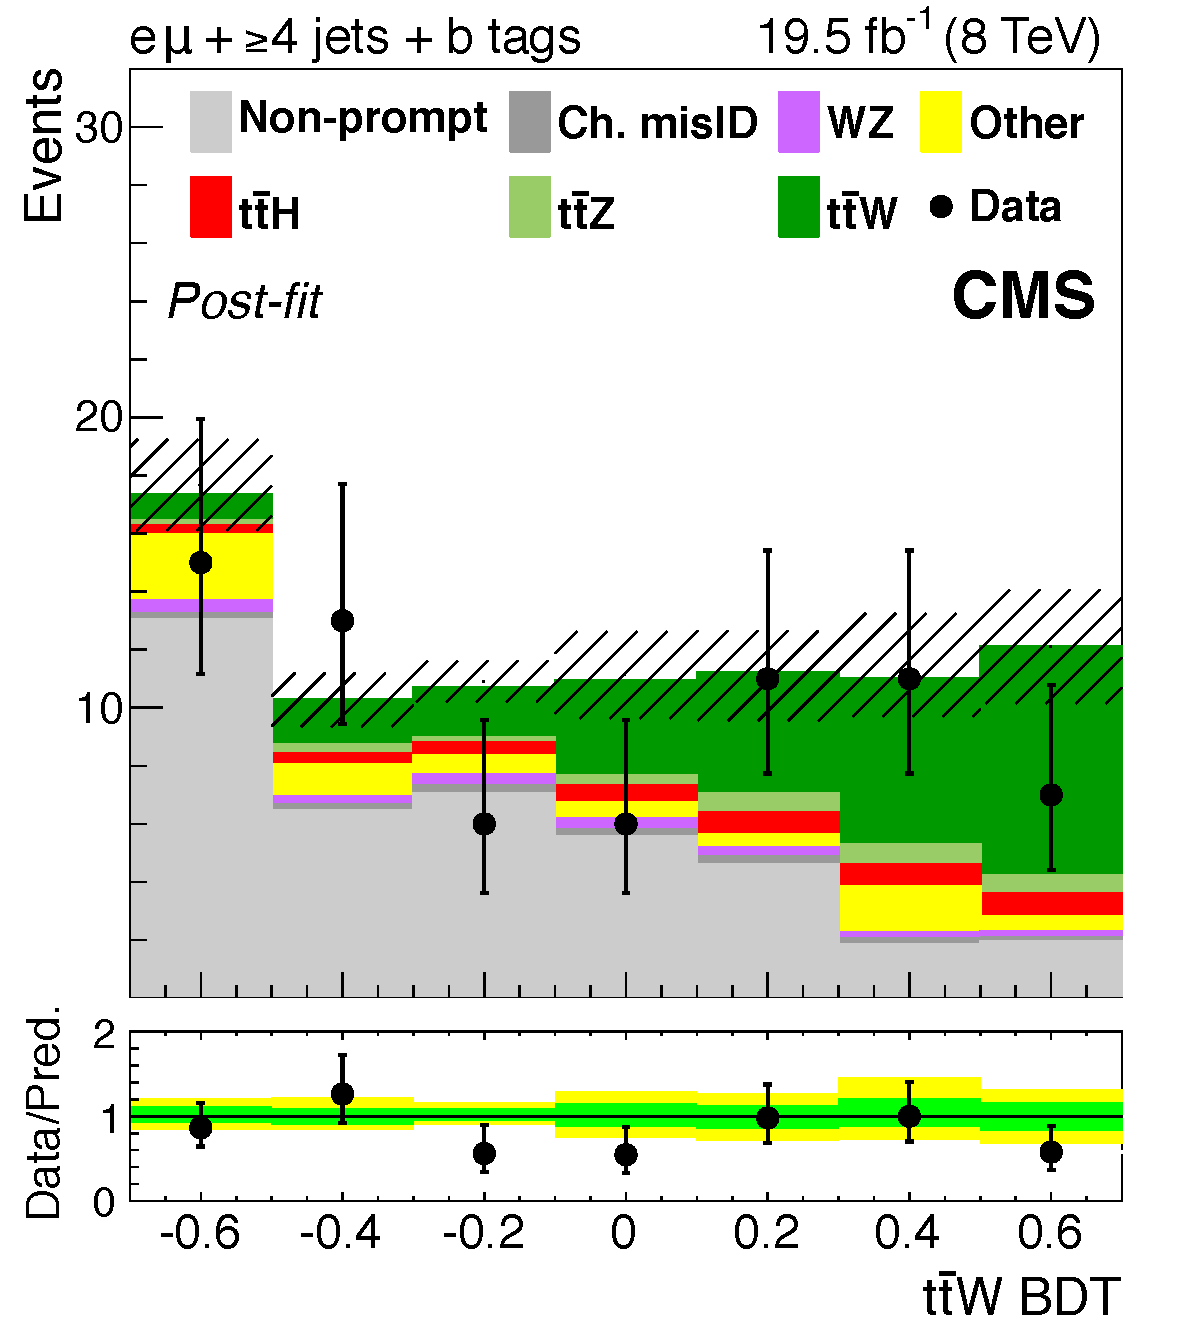
\includegraphics[width=\textwidth]{figures/eight-TeV/mva/mu_ele_ge4j_bloose_FinalBDT}
    \caption{}
    \label{sfig:8-ttW-cc}
  \end{subfigure}%
  \begin{subfigure}{0.33\textwidth}
    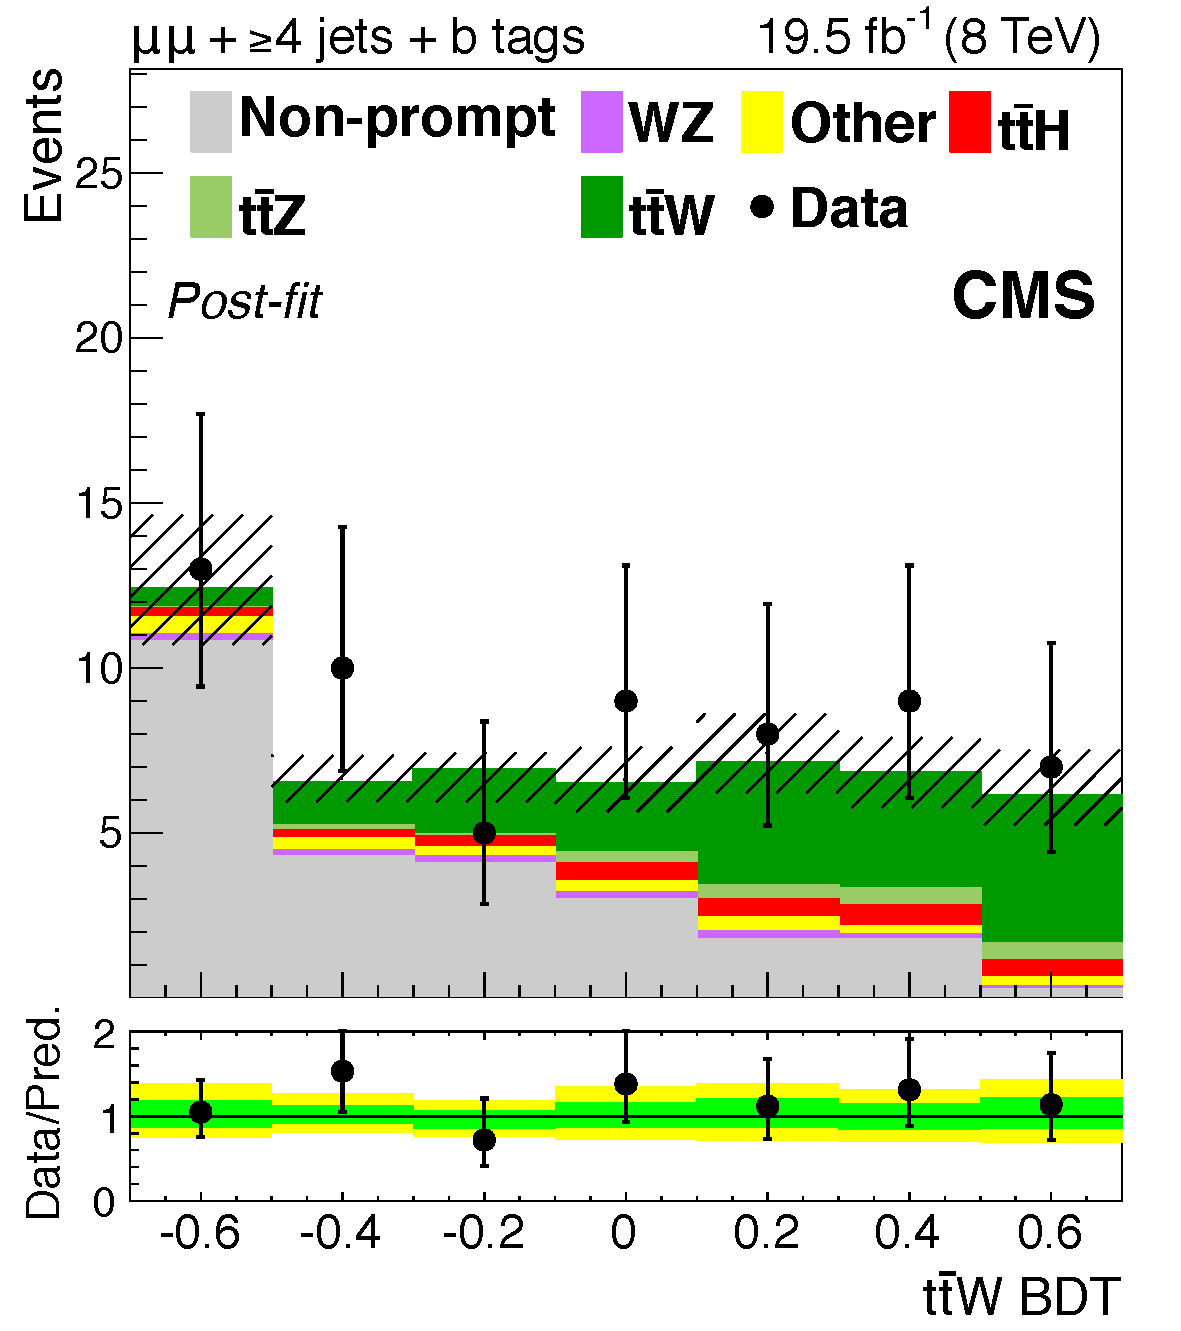
\includegraphics[width=\textwidth]{figures/eight-TeV/mva/mu_mu_ge4j_bloose_FinalBDT}
    \caption{}
  \end{subfigure}
  \begin{subfigure}{0.33\textwidth}
    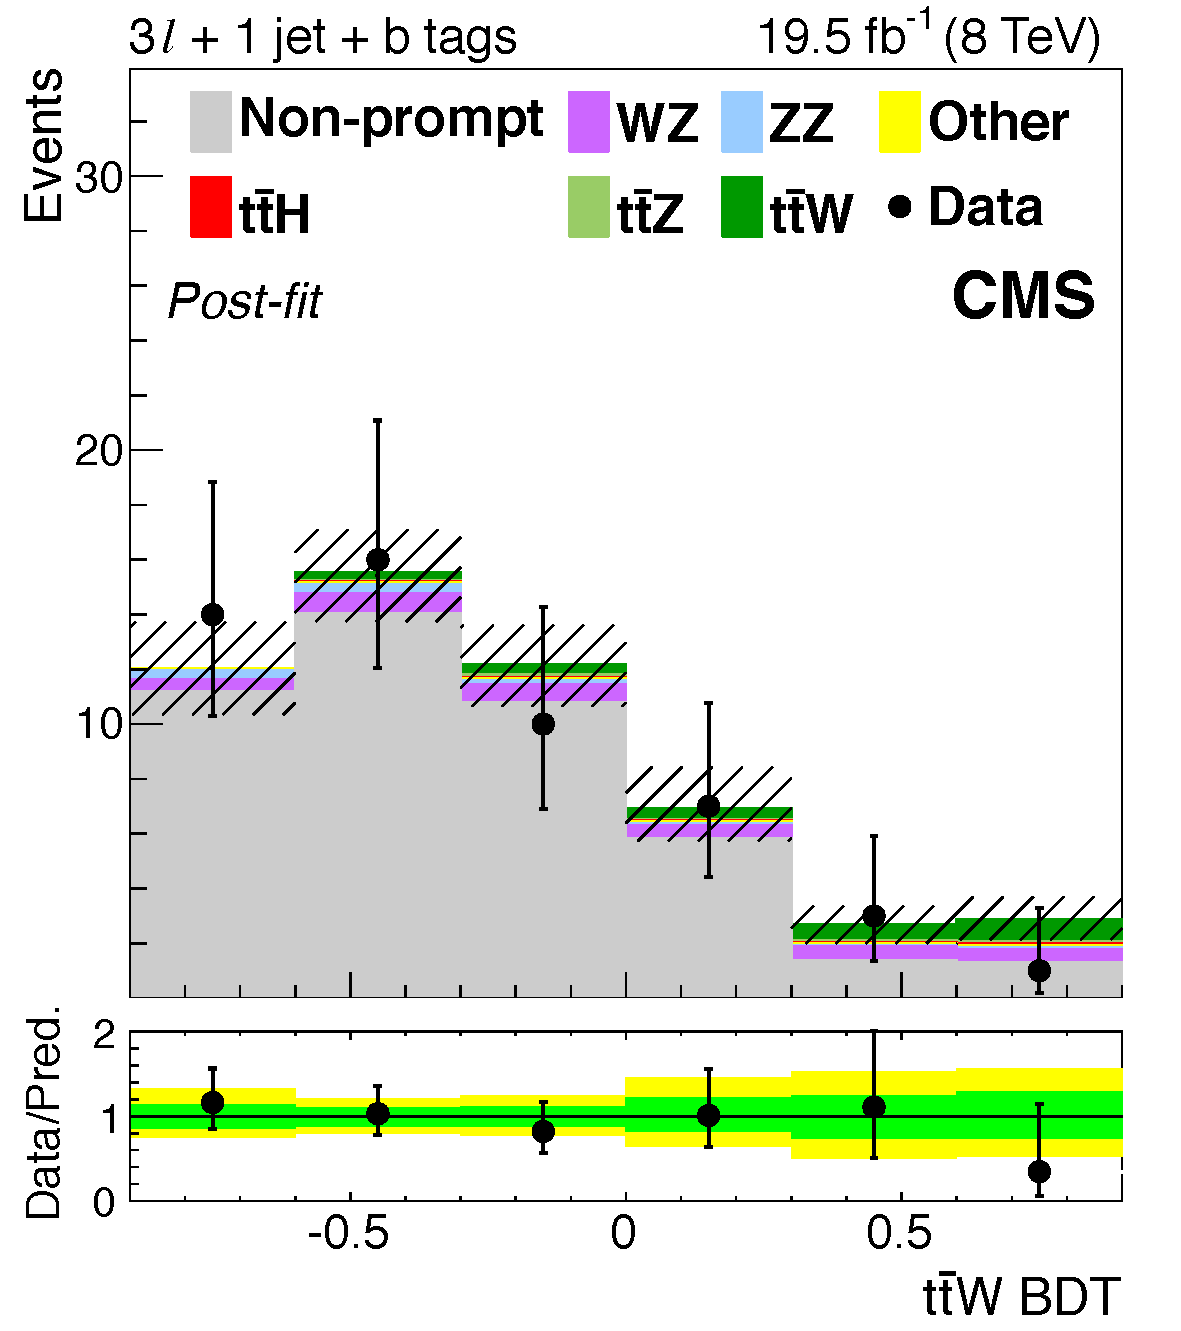
\includegraphics[width=\textwidth]{figures/eight-TeV/mva/3l_eq1j_bloose_FinalBDT}
    \caption{}
    \label{sfig:8-ttW-bl}
  \end{subfigure}
  \begin{subfigure}{0.33\textwidth}
    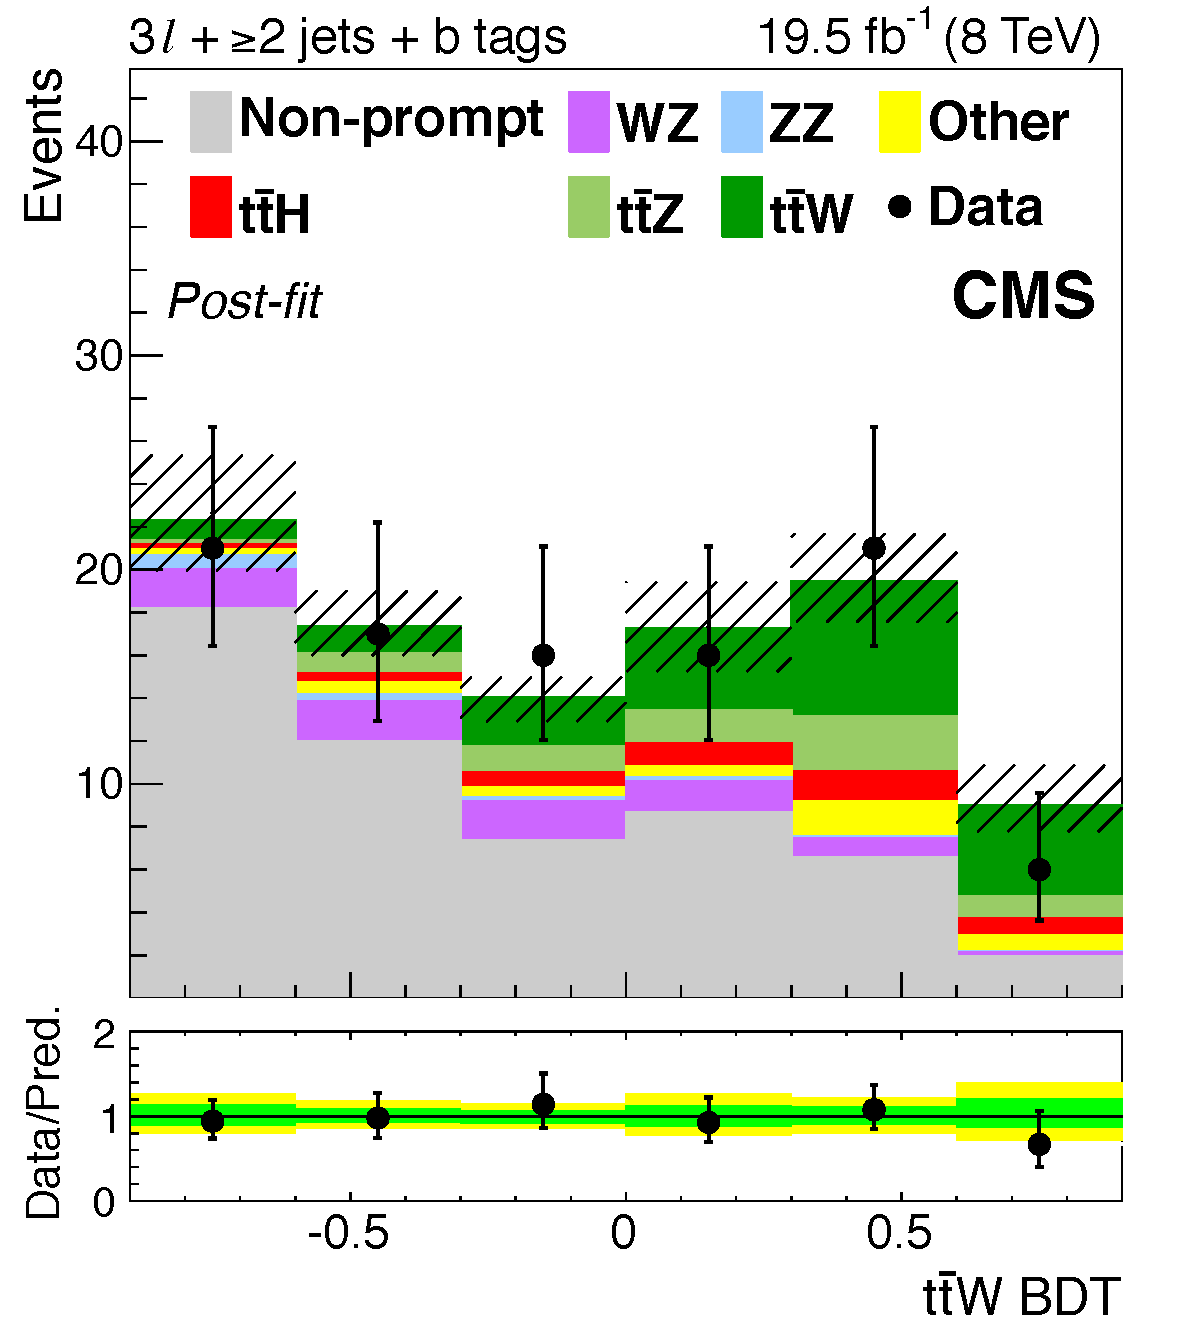
\includegraphics[width=\textwidth]{figures/eight-TeV/mva/3l_ge2j_bloose_FinalBDT}
    \caption{}
    \label{sfig:8-ttW-br}
  \end{subfigure}
  \vspace{-1cm}
  \caption[Final discriminant for events in the \ttW channel]{
    The post-fit final discriminant for events in the SS \ttW channel with 3 jet (top row) and
    $\geq$4 jets (center row), for lepton flavors $\Pe\Pe$ (a, d), $\Pe\mu$ (b, e), and $\mu\mu$ (c,
    f). The post-fit final discriminant for events in the 3\lep \ttW channel with 1
    jet~\subref{sfig:8-ttW-bl} and $\geq$2 jets~\subref{sfig:8-ttW-br}. The hashed regions in the
    stack histogram indicate \SI{68}{\percent} CL uncertainty on the signal plus background. The
    green and yellow shaded regions on the data-to-prediction ratio plot indicate \SI{68}{\percent}
    and \SI{95}{\percent} CL bands, respectively.
  }
  % ``Ch.~misID'' indicates the charge-misidentified background. ``Other'' backgrounds include $\ttbar\gamma$, $\ttbar\gamma^{*}$, $\ttbar\PW\PW$, tb$\cPZ$, WWW, WWZ, and W$^{\pm}$W$^{\pm}$.}
  \label{fig:8-postfit-bdt-ttW}
\end{figure}
\begin{figure}[tb]
  \centering
  \begin{subfigure}{0.33\textwidth}
    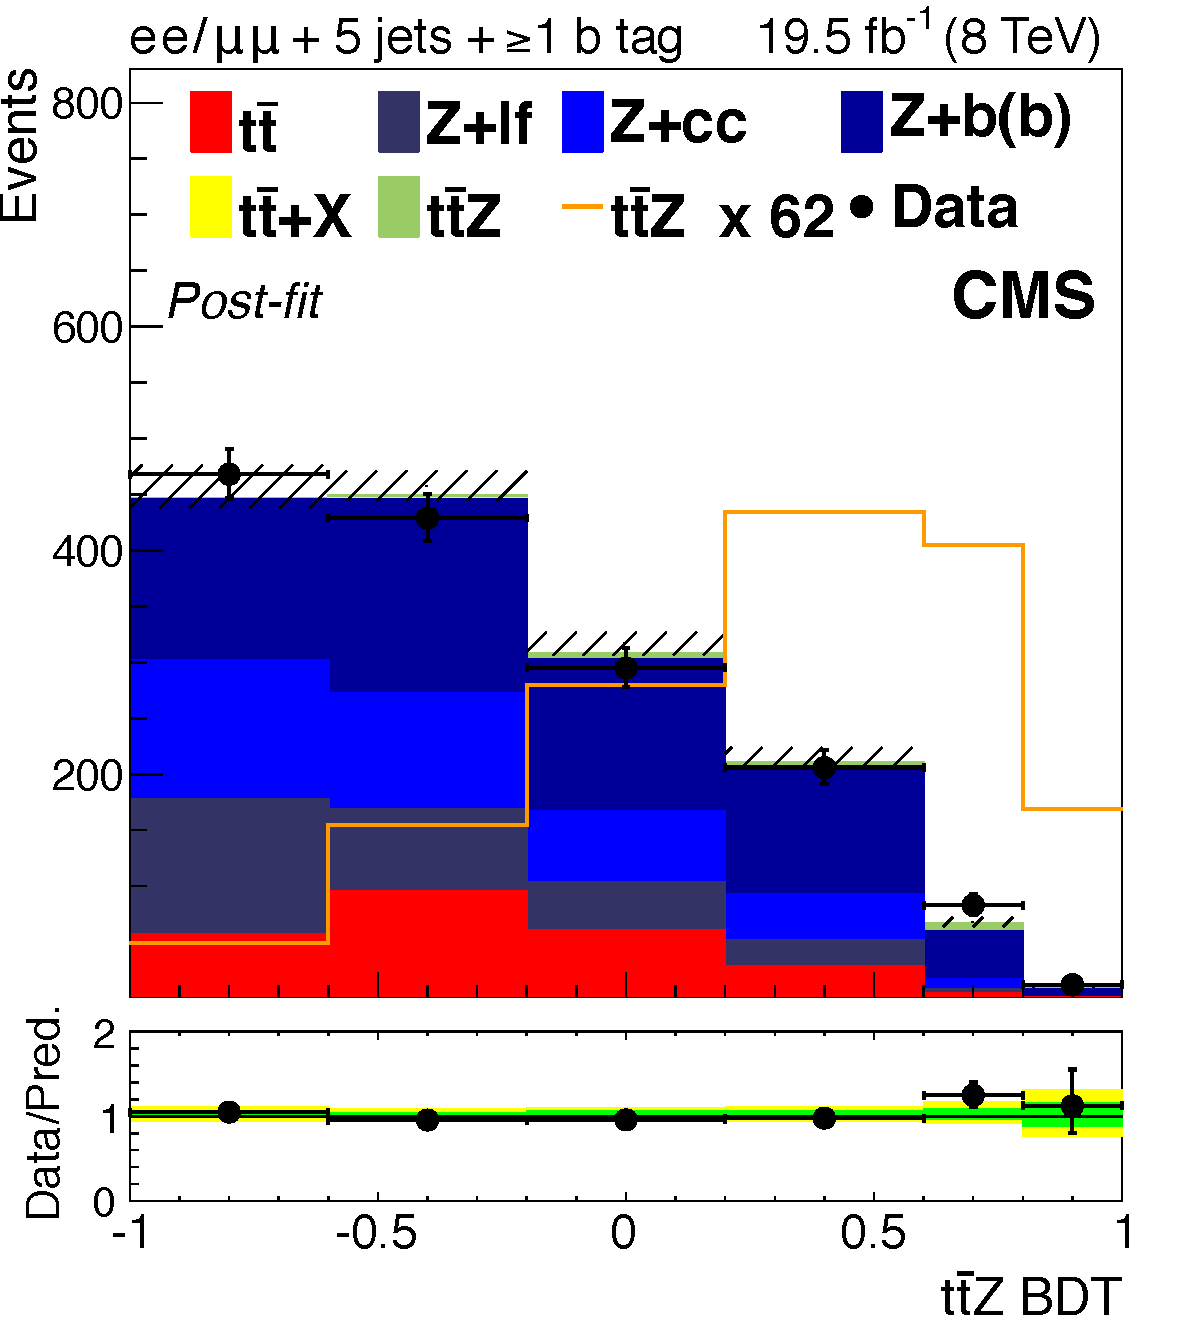
\includegraphics[width=\textwidth]{figures/eight-TeV/mva/lep_lep_SF_eq5j_ge1t_FinalBDT}
    \caption{}
    \label{sfig:8-ttZ-tl}
  \end{subfigure}%
  \begin{subfigure}{0.33\textwidth}
    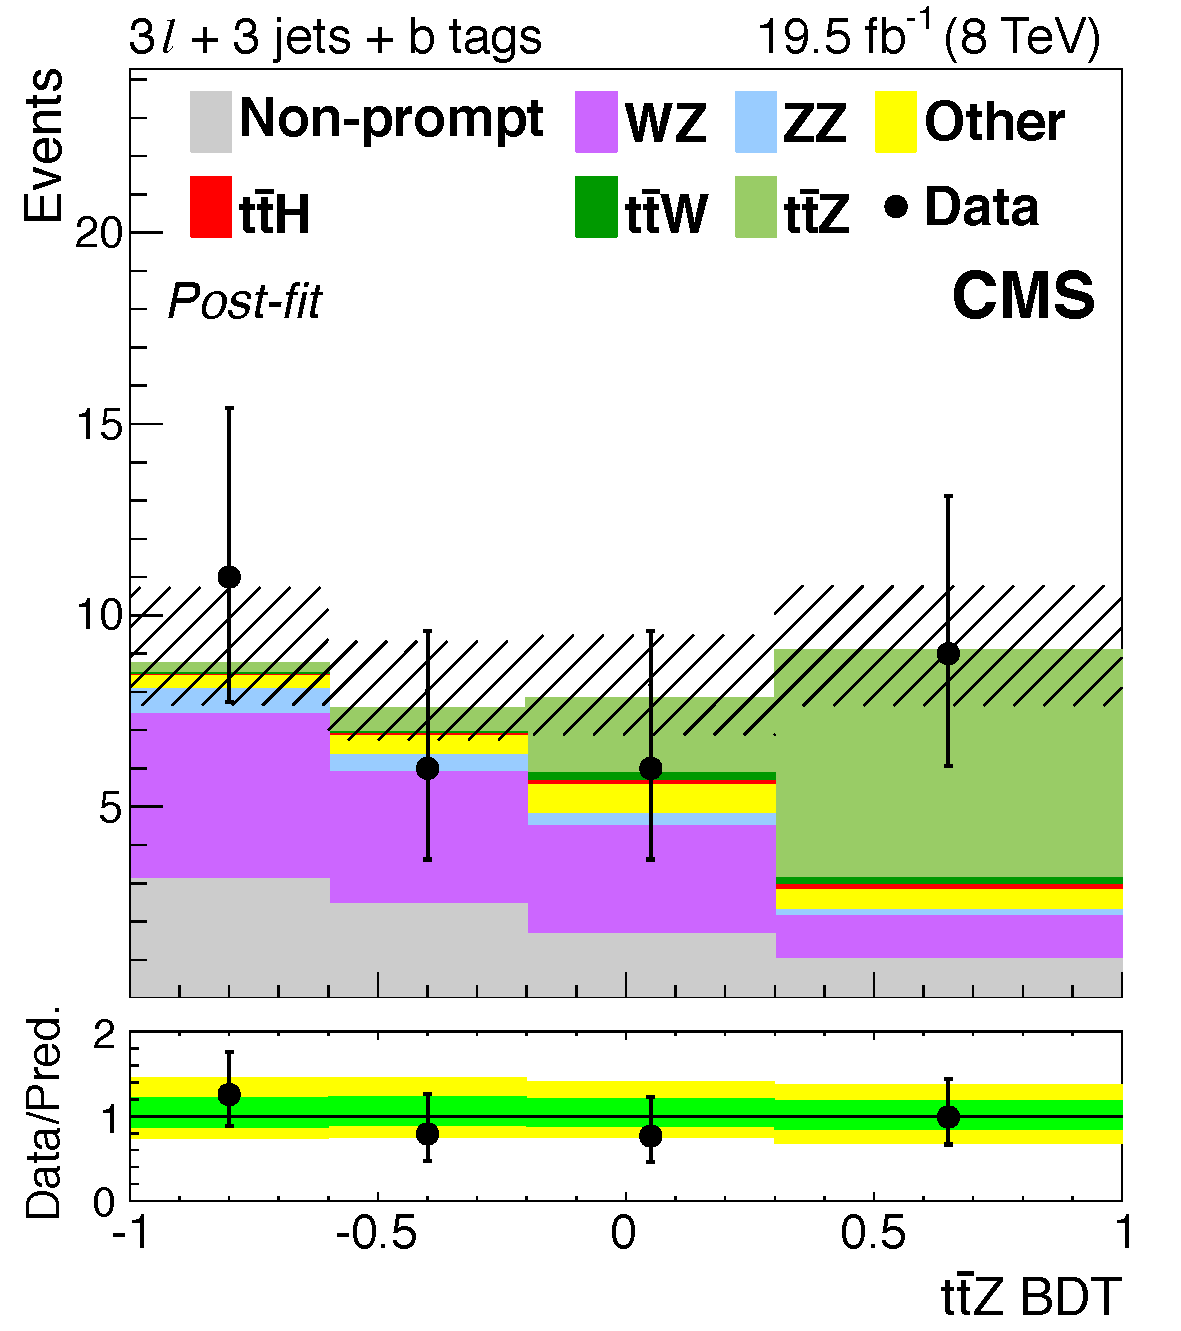
\includegraphics[width=\textwidth]{figures/eight-TeV/mva/3l_eq3j_bloose_FinalBDT}
    \caption{}
    \label{sfig:8-ttZ-tc}
  \end{subfigure}%
  \begin{subfigure}{0.33\textwidth}
    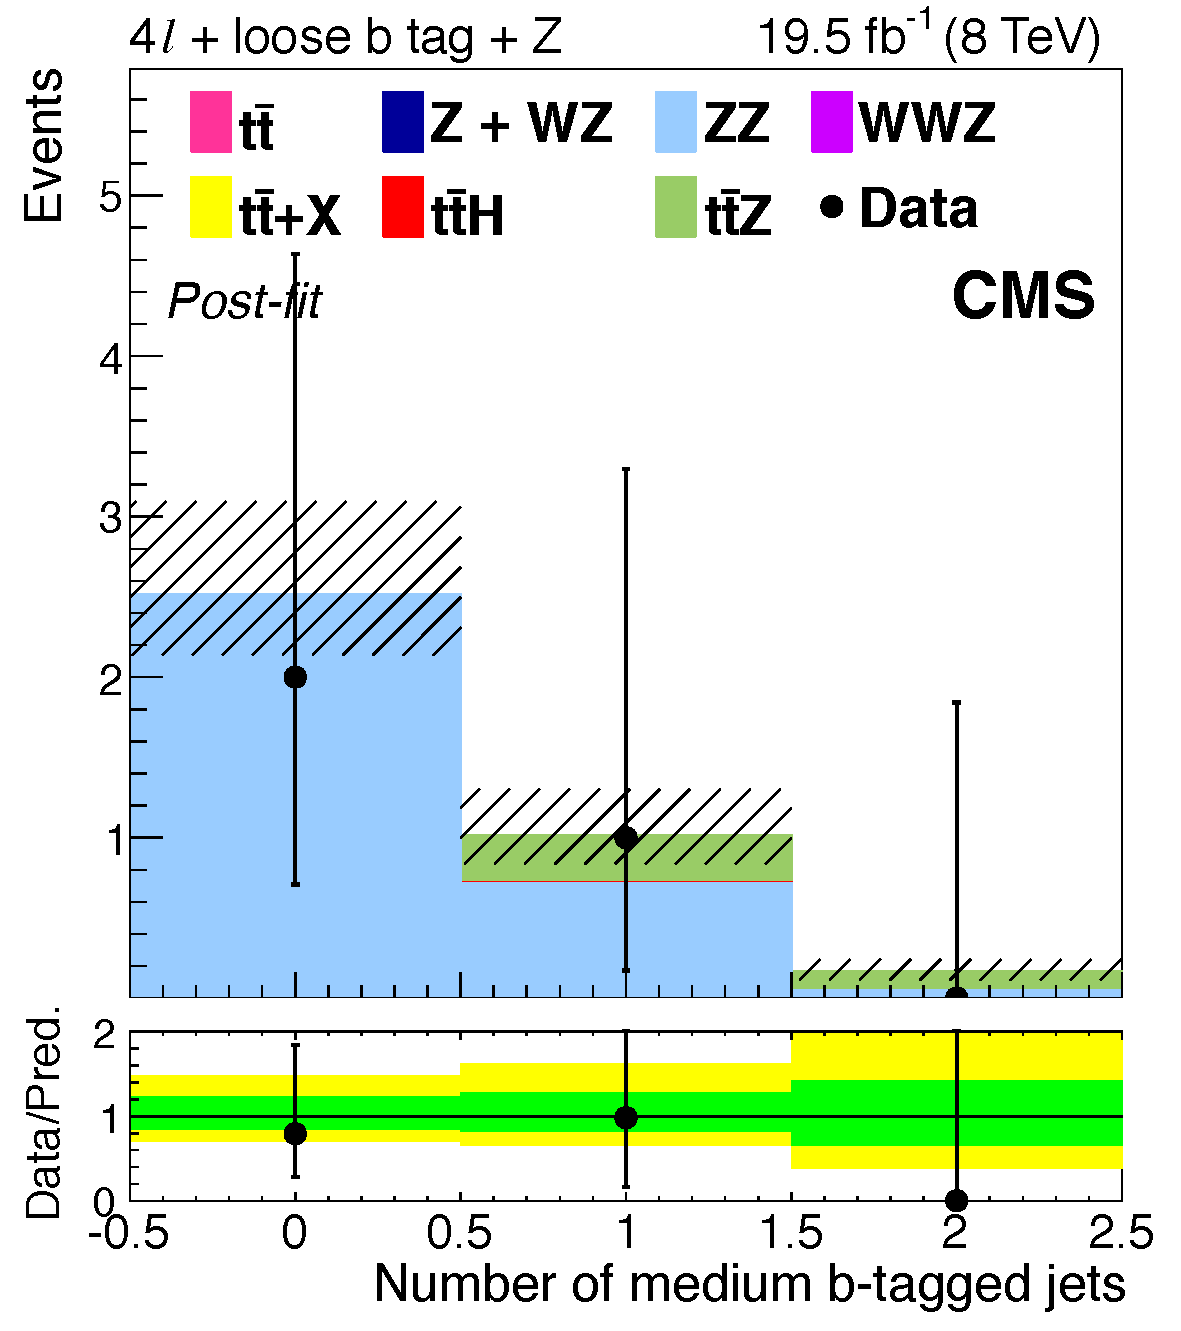
\includegraphics[width=\textwidth]{figures/eight-TeV/mva/4l_ge1j_Zpeak_mht30_1bloose_numMediumBJets}
    \caption{}
    \label{sfig:8-ttZ-tr}
  \end{subfigure}
  \begin{subfigure}{0.33\textwidth}
    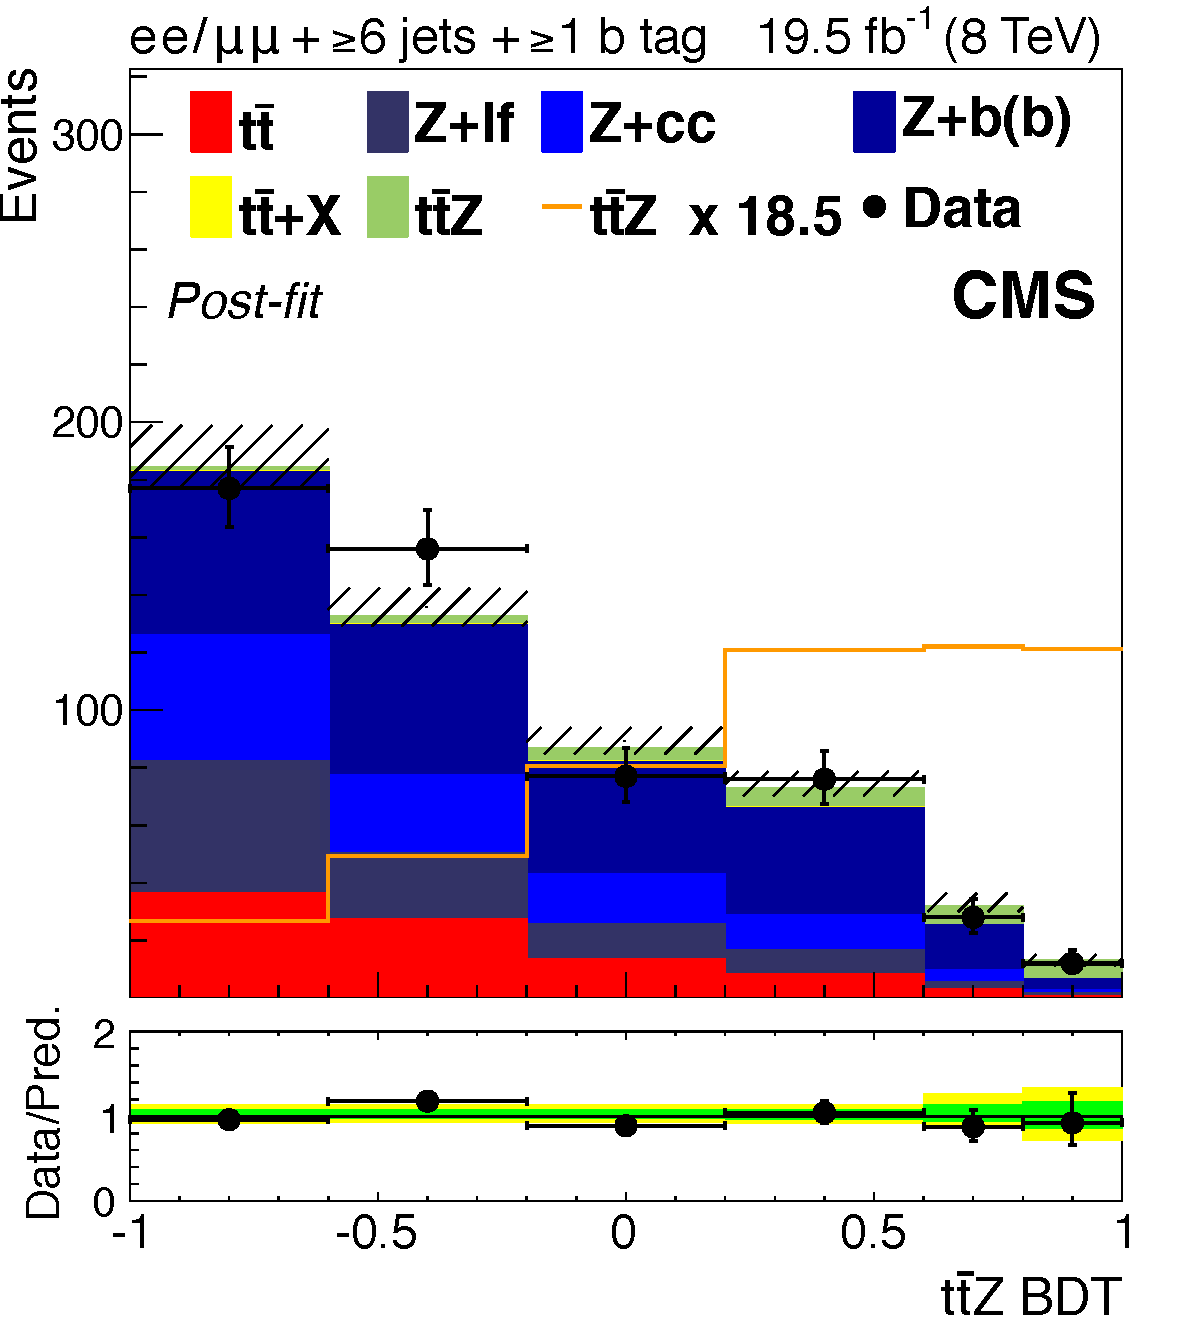
\includegraphics[width=\textwidth]{figures/eight-TeV/mva/lep_lep_SF_ge6j_ge1t_FinalBDT}
    \caption{}
    \label{sfig:8-ttZ-bl}
  \end{subfigure}%
  \begin{subfigure}{0.33\textwidth}
    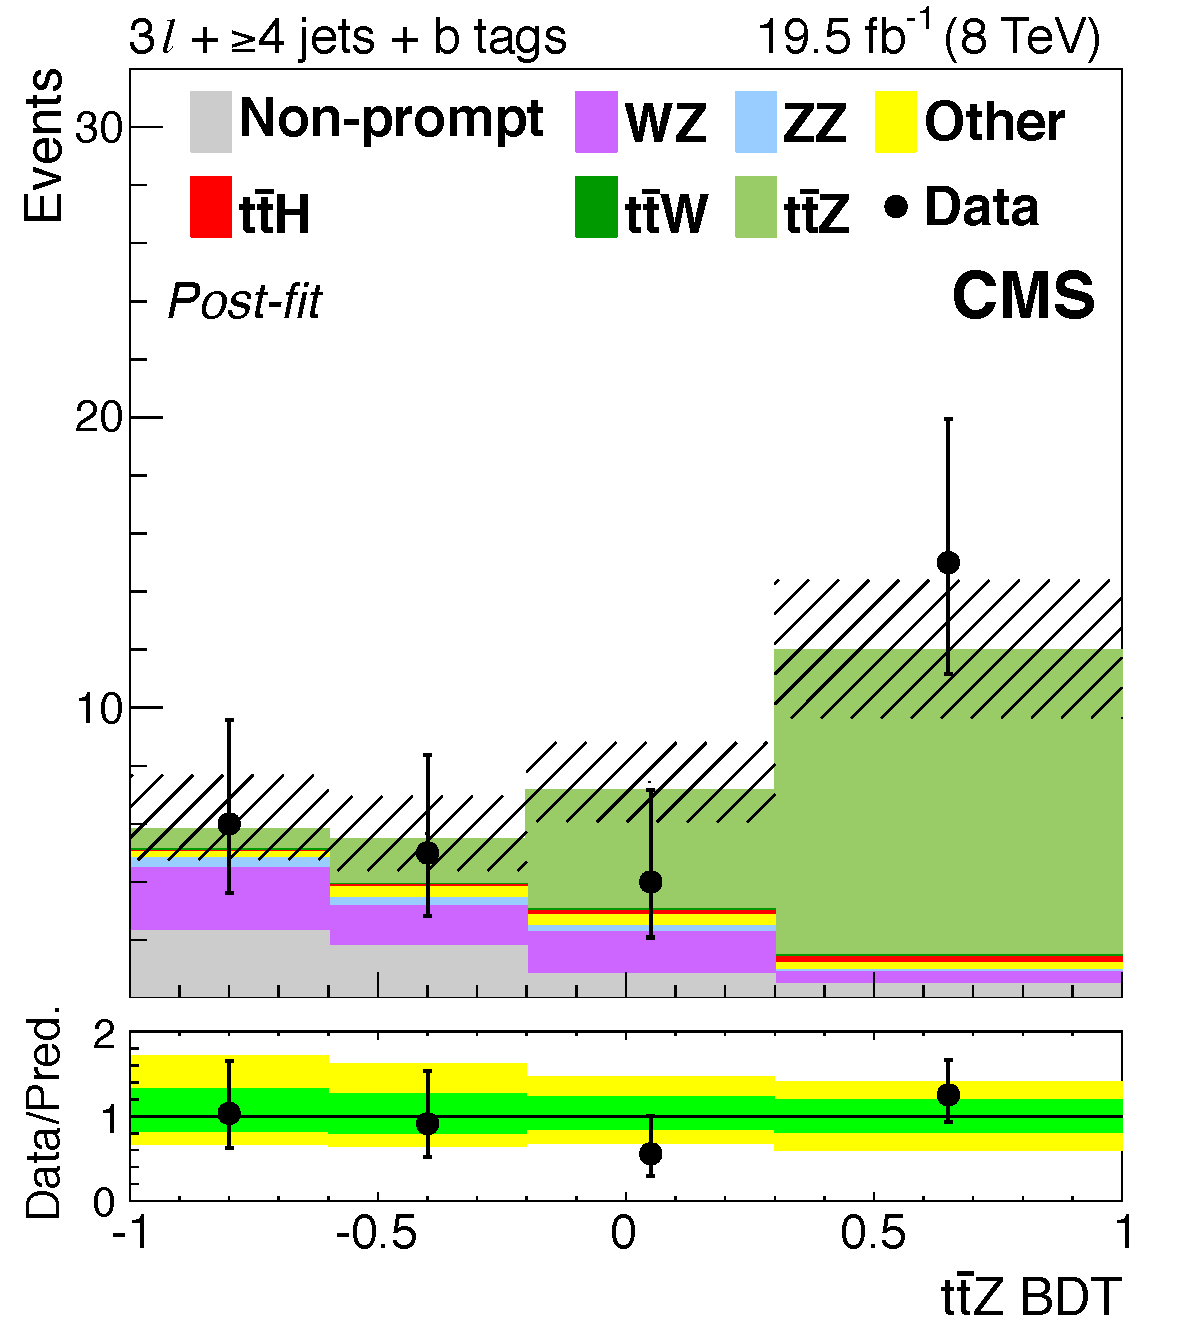
\includegraphics[width=\textwidth]{figures/eight-TeV/mva/3l_ge4j_bloose_FinalBDT}
    \caption{}
  \end{subfigure}%
  \begin{subfigure}{0.33\textwidth}
    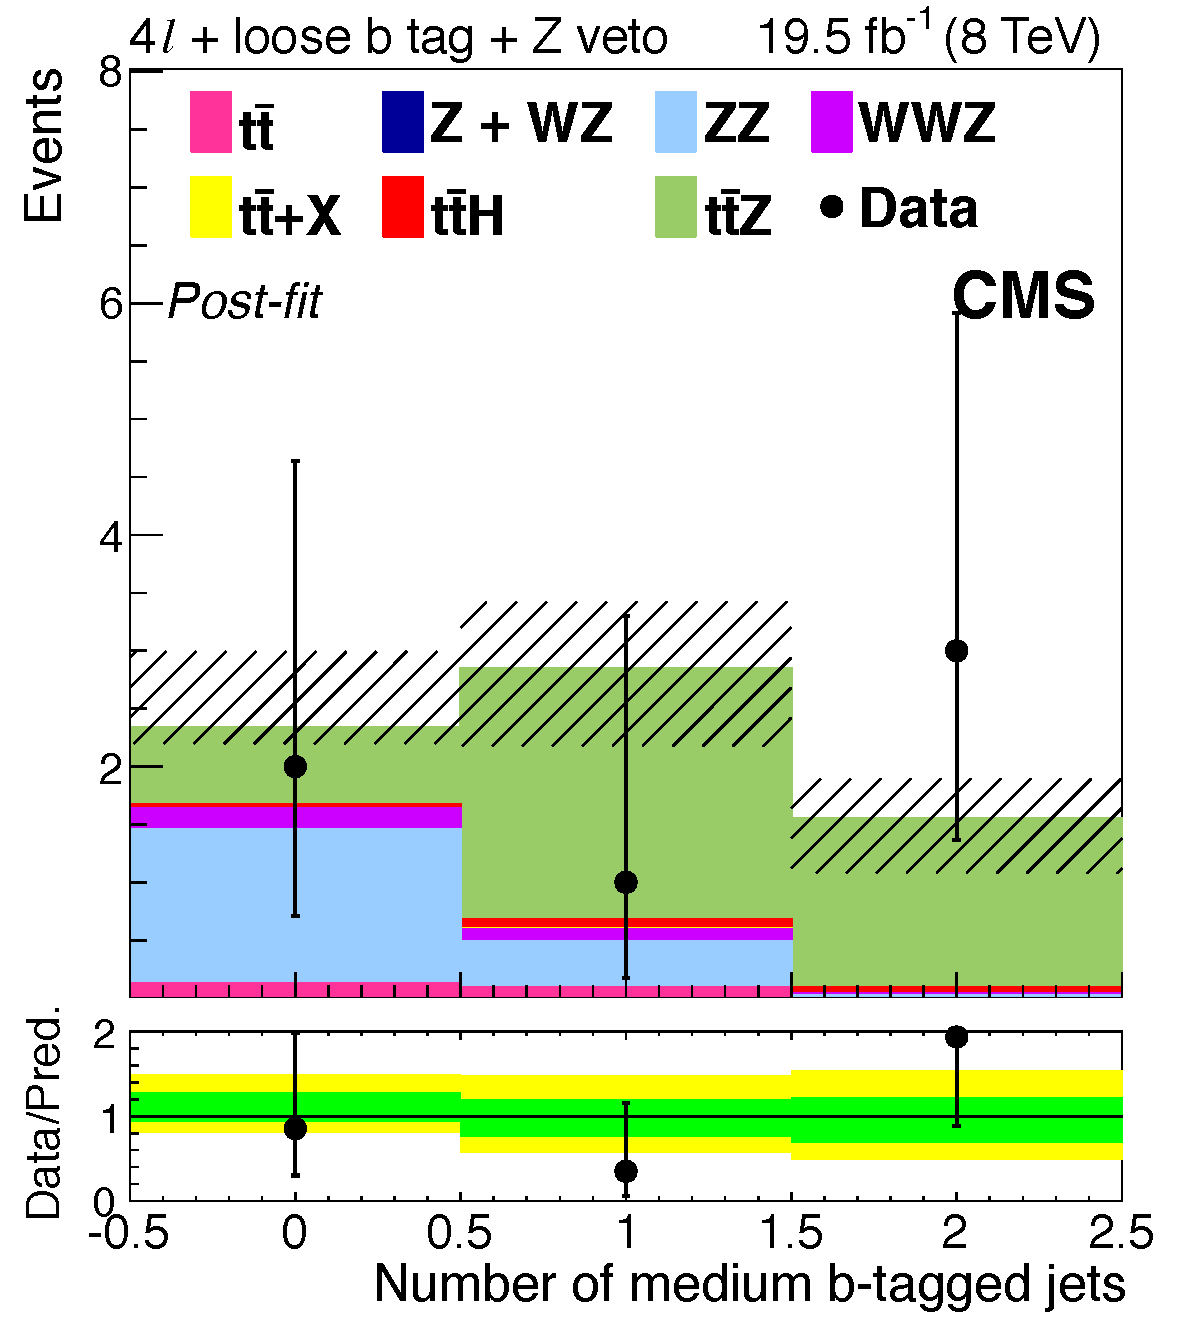
\includegraphics[width=\textwidth]{figures/eight-TeV/mva/4l_ge1j_Zmask_mht30_1bloose_numMediumBJets}
    \caption{}
  \end{subfigure}%
  \caption[Final discriminant for events in the \ttZ channel]{
    The post-fit final discriminant for events in the OS \ttZ channel with two
    OS leptons and 5 jets (a) or $\geq$6 jets (d), three leptons and 3 jets (b)
    or $\geq$4 jets (e), or four leptons and two lepton pairs (c) or exactly one
    lepton pair (f) consistent with a $\PZ \rightarrow \ell\ell$ decay. The
    hashed regions in the stack histogram indicate \SI{68}{\percent} CL
    uncertainty on the signal plus background. The green and yellow shaded
    regions on the data-to-prediction ratio plot indicate \SI{68}{\percent} and
    \SI{95}{\percent} CL bands, respectively.
  }
  % The $\ttbar$+X background includes $\ttW$, $\ttH$, and $\ttbar\PW\PW$; ``Other'' backgrounds include $\ttbar\gamma$, $\ttbar\gamma^{*}$, $\ttbar\PW\PW$, tb$\cPZ$, WWW, and WWZ.}
  \label{fig:8-postfit-bdt-ttZ}
\end{figure}

\begin{figure}[tb]
  \centering
  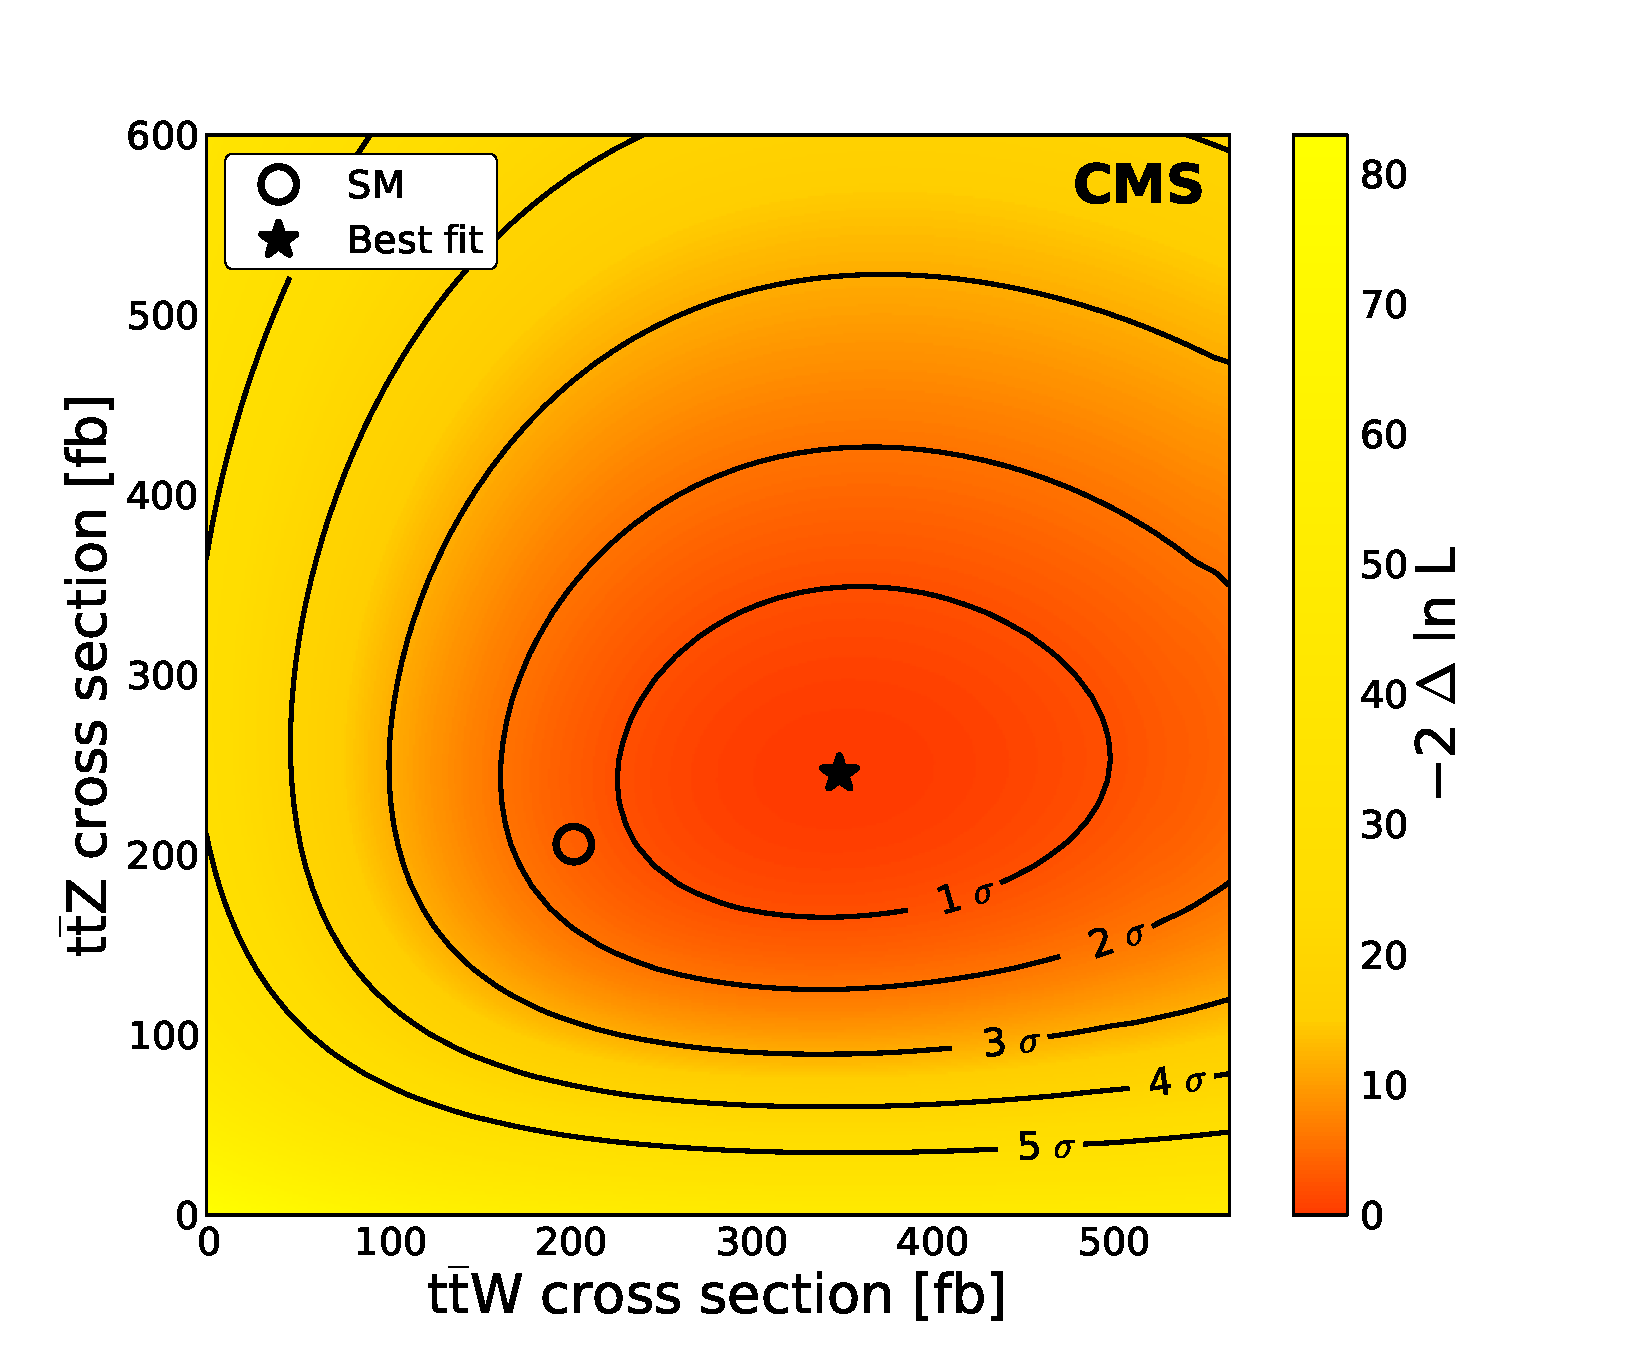
\includegraphics[width=0.8\textwidth]{figures/eight-TeV/z_color_map_and_contour_5_sigma_ttZ_ttW_2d_v4_all_stats}
  \caption[Profile likelihood for simultaneous fit as a function of
  $\sigma_{\ttZ}$ and $\sigma_{\ttW}$]{Profile likelihood as a function of
    $\sigma_{\ttW}$ and $\sigma_{\ttZ}$. Lines denote the 1 to 5 standard
    deviation ($\sigma$) CL contours.
  }
  \label{fig:8-2d-ttZ-ttW}
\end{figure}
